\chapter{Modeling Carbon Dioxide Vibrational Frequencies in Ionic Liquids: I. \textit{Ab Initio} Calculations}
\label{ch:paper_02}

Eric J. Berquist,\textsuperscript{1,2} Clyde A. Daly Jr.,\textsuperscript{3} Thomas Brinzer,\textsuperscript{1,2} Krista K. Bullard,\textsuperscript{1,2} Zachary M. Campbell,\textsuperscript{1,2} Steven A. Corcelli,\textsuperscript{3} Sean Garrett-Roe,\textsuperscript{1,2} and Daniel S. Lambrecht\textsuperscript{1,2*}

\textsuperscript{1}Department of Chemistry, University of Pittsburgh, 219 Parkman Ave, Pittsburgh, Pennsylvania. \textsuperscript{2} Pittsburgh Quantum Institute. \textsuperscript{3}Department of Chemistry and Biochemistry, University of Notre Dame, Notre Dame, Indiana.

\section{\caps{Summary}}
\label{paper_02:sec:summary}

This work elucidates the molecular binding mechanism of \ce{CO2} in \ce{[C4C1im][PF6]} ionic liquid (IL) and its interplay with the \ce{CO2} asymmetric stretch frequency \(\nu_{3}\), and establishes computational protocols for the reliable construction of spectroscopic maps for simulating ultrafast 2D-IR data of \ce{CO2} solvated in ILs. While charge transfer drives the static frequency shift between \emph{different} ionic liquids {[}\emph{J. Chem. Phys.}  \textbf{142}, 212425 (2015){]}, we find here that electrostatic and Pauli repulsion effects dominate the dynamical frequency shift between different geometries sampled from the finite-temperature dynamics within a single ionic liquid. This finding is also surprising because dispersion interactions dominate the \ce{CO2}\textendash{}IL interaction energies, but are comparably constant across different geometries. An important practical consequence of this finding is that density functional theory is expected to be sufficiently accurate for constructing potential energy surfaces for \ce{CO2} in \ce{[C4C1im][PF6]}, as needed for accurate anharmonic calculations to construct a reliable spectroscopic map. Similarly, we established appropriate computational and chemical models for treating the extended solvent environment. We found that a QM/MM treatment including at least \num{2} cation-ion pairs at the QM level and at least \num{32} pairs at the MM level is necessary to converge vibrational frequencies to within \SI{1}{\wavenumber}. Using these insights, this work identifies a computational protocol as well as a chemical model necessary to construct accurate spectroscopic maps from first principles.

\section{\caps{Introduction}}
\label{paper_02:sec:I}

Capturing anthropogenic \ce{CO2} before its release into the atmosphere is a pressing need, and most methods will require the development of novel materials, such as metal-organic frameworks, polymers, or ionic liquids (ILs).\cite{sumidaCR-12,Du2011,Dawson2011,baraACR-10,seoJPCB-14,DAlessandro2010} Understanding how to control the interactions between \ce{CO2} and its condensed-phase environment is a key to achieving efficient carbon capture and sequestration\cite{Corvo2015,Hayes2015,seoJPCB-14,gurkanJPCL-10} and to developing routes toward potentially transforming \ce{CO2} into value-added chemicals including fuels.\cite{Grice2015,Rosen2011,Kumar2012} To rationally develop such technologies, a molecular level understanding of the \ce{CO2}-sorbent interactions, structures and dynamics is necessary.

In a previous paper\cite{Brinzer2015}, some of us established that \ce{CO2}'s asymmetric vibrational stretch mode (\(\nu_{3}\)) can be used to effectively probe the structure and dynamics of \ce{CO2} dissolved in ILs. Using a combination of ultrafast two-dimensional infrared (2D-IR) spectroscopy and computational modeling, we determined structural candidates for the immediate \ce{CO2} solvent environments whose vibrational solvation shifts were consistent between experiment and theory. Experimentally, the timescales of structural reorganization relative to the \ce{CO2} molecule were correlated to the bulk viscosity. This experimental correlation between molecular property (solvation timescales) and bulk property (viscosity) suggests that \ce{CO2} motions are gated by the same motions that lead to bulk diffusion. Molecular models are needed, however, to establish physical explanations for the correlation.

\ce{CO2} solvation in ionic liquids gives rise to several interesting and challenging effects that are worth exploring thoroughly, taking both computational methodology and the chemical picture into account. Our previous work suggested that charge transfer (CT) between \ce{CO2} and the IL dominates the differentiation of the calculated vibrational signatures between different ionic liquids. Understanding the strength and nature of intermolecular interactions between \ce{CO2} and its IL solvent fundamentally shapes our model of the \ce{CO2}\textendash{}IL interaction. Investigating \ce{CO2}\textendash{}IL interactions will thus deepen our understanding of the mechanism of \ce{CO2} solubility in ionic liquids, and even of (de)activation of \ce{CO2} for catalytic reductions. Interestingly, the asymmetric stretch frequency of \ce{CO2} encodes the strength of intermolecular interactions as they are manifested in the molecular geometry of \ce{CO2} interacting with the surrounding IL. In other words, one can determine the correct vibrational frequency shift for \ce{CO2} from the distortion of the \ce{CO2} geometry, but correctly determining the \ce{CO2} geometry requires an understanding of intermolecular interactions between \ce{CO2} and the IL solvent. These effects must be considered in the development of more reliable force fields that describe \ce{CO2}\textendash{}IL solvation, and of empirical structure-spectra maps used for comparing MD results with results from ultrafast spectroscopies.

This publication is first in a series aiming to unravel the physics underlying \ce{CO2}\textendash{}IL interactions as probed via vibrational spectroscopy and to develop a spectroscopic map to facilitate simulation of these spectra. \emph{The central point of the present publication is to establish a more refined picture of intermolecular interactions and their correlations with vibrational shifts by improving both the computational approach and the chemical model as described below.} Some of the results from this publication inform the method choices for the subsequent paper in the series, where we develop and validate a spectroscopic map enabling one to reliably predict both the position and the width of the \ce{CO2} asymmetric vibrational peak within classical MD simulations.\cite{Daly2016}

In this manuscript, we address the critical challenges needed to generalize our previous work. The key issues are: treating the condensed phase environment, testing the dependence on the electronic structure theory method and basis set, and addressing anharmonic effects.

First, we extend our previous results by analyzing both the convergence and stability of the calculations with respect to the computational approach. Our absolutely localized molecular orbital (ALMO) calculations\cite{Khaliullin2006,Khaliullin2007,Khaliullin2008} evaluated the impact of CT and other chemically intuitive components in the calculation of spectral signatures by using the modest B3LYP/6-31G(d,p) level of theory. Like most decomposition approaches, the ALMO results are expected to show some dependence on the underlying density functional approximation; in particular, it is known that the predicted amount of charge transfer depends on the amount of self-interaction error (SIE) present and the resulting (spurious) delocalization\cite{Ramos-Cordoba2011}. As a result, non-SIE corrected functionals are expected to overestimate the amount of CT, whereas the SIE-free Hartree\textendash{}Fock approach can be used to estimate a lower bound for CT effects. Likewise, one can expect the CT contribution to depend on the basis set diffuseness, since the ALMO definition of CT is closely linked to the penetration of basis functions between different fragments. Thus, one goal of the present study is to quantify the method and basis set dependence of the calculated vibrational shifts and their effect on CT.

Although our previous density functional theory (DFT) calculations provided excellent agreement of predicted vibrational solvation shifts compared to experiment, these employed a minimalistic gas-phase cluster model consisting of only one \ce{CO2} molecule together with a single cation/anion pair. Here we investigate the convergence of results with the size of the surrounding solvent shell both using a hybrid quantum mechanics molecular mechanics (QM/MM) approach with up to \num{195} atoms (\num{6} molecular ion pairs) in the QM region and up to \num{8192} solvent atoms (\num{256} molecular ion pairs) using classical point charges. In addition, we aim to assess the impact of solvent disorder by investigating different solvent geometries based on \num{85} statistically uncorrelated (\(R^2 = 0.0004\) for DVR-based vibrational frequency of snapshot \(N\) to vibrational frequency of snapshot \(N+1\)) snapshots sampled from a classical MD simulation (see paper II\cite{Daly2016} for details). We use 1-butyl-3-methylimidazolium hexafluorophosphate (\ce{[C4C1im][PF6]}) as a model IL in our calculations.

We will further analyze the impact of anharmonic effects, which we neglected in our previous (harmonic) calculations and which are necessary for a fair comparison to experiment. Here, anharmonic vibrational frequencies are obtained using the discrete variable representation (DVR) approach. The DVR method numerically solves the vibrational Schr\"{}odinger equation using a calculation of the \ce{CO2} stretch potential energy surface, resulting in vibrational frequencies that include anharmonicity to all orders. An additional advantage of DVR is that it can be applied rigorously to systems at non-equilibrium geometries, which allows us to include the disorder introduced by temperature for comparison with experiments carried out at temperatures above absolute zero.

The energy decomposition approaches we use add new and valuable physical insight into the origin of the vibrational frequency shifts. Many groups have used QM/MM approaches to estimate the condensed phase effects of a solvent on the transition energies of a chromophore, which provide a rich interpretation of the experiments\cite{choiJCP-08,Lindquist2008,Terranova2014,liJPC-06,Schmidt2008}. Nevertheless, the interpretation for why the environment shifts the transition frequencies is difficult because many effects simultaneously determine the transition frequencies. The ALMO and symmetry-adapted perturbation theory (SAPT) energy decomposition approaches can separate the interactions of the vibrational chromophore with its environments into meaningful components allowing us to develop an empirical spectroscopic map and also understand its physical origins.

The paper is organized as follows. In section~\ref{paper_02:sec:II}, we give a detailed account of the computational approaches used, including DFT calculations and DVR vibrational frequency calculations. In section~\ref{paper_02:sec:III}, we analyze the dependence of the calculated \ce{CO2} vibrational frequencies on the computational approach and the chemical model. For the computational approach, we quantify both the impacts of the electronic structure method (density functional and basis set) as well as the inclusion of anharmonic effects via the DVR approach. We analyze the dependence on the chemical model by comparing our previous gas-phase cluster calculations with results obtained for extended solvent boxes both at the classical point charge and the hybrid quantum mechanics/molecular mechanics (QM/MM) level, where structures are sampled from extensive molecular dynamics (MD) simulations (details of the MD simulations will be discussed in a follow-up paper\cite{Daly2016}). This way, we aim to include the most important effects of solvent electrostatics, exchange-repulsion, and solvent disorder. In section~\ref{paper_02:sec:IV} we present concluding remarks and an outlook for future research.

\section{\caps{Computational Methods}}
\label{paper_02:sec:II}

\subsection{Methods and Basis Sets}
\label{paper_02:ssec:IIA}

Similar to our previous work\cite{Brinzer2015}, we choose gas-phase clusters consisting of one \ce{[C4C1im][PF6]} ion pair with \ce{CO2} to quantify the effects of quantum chemical method and basis set on the quantum mechanically calculated harmonic frequencies. For methods, we employ the BLYP\cite{Becke1988,Lee1988} generalized gradient approximation (GGA) and B3LYP\cite{Becke1993,Stephens1994} hybrid GGA density functionals, along with Hartree\textendash{}Fock (HF) theory. This choice of methods allows us to test the dependence of the results on the percentage of exact (HF) exchange, as these methods have 0\%, 20\%, and 100\% HF exchange, respectively. For basis sets, we choose 6-31G(d,p)\cite{Hehre1972,Francl1982} and 6-311++G(d,p)\cite{Krishnan1980,McLean1980,Clark1983} to represent the commonly-used Pople-style basis sets (abbreviated as ``small Pople'' [SP] and ``large Pople'' [LP] in the following), along with Dunning's correlation-consistent basis sets from double- to quadruple-\(\zeta\) quality (cc-pVXZ, where X = D,T,Q, abbreviated as VXZ)\cite{Dunning1989,Dunning1993}. Initial geometries were constructed using Avogadro\cite{Hanwell2012,Avogadro} before optimization to local minima with or without charge transfer allowed between molecules (\latin{vide infra}), followed by harmonic frequency calculations.

To examine solvent effects, we investigate the converge of QM-calculated harmonic frequencies as a function of the solvent box size, where we vary both the number of ionic liquid pairs treated explicitly (``QM pairs'') and treated as point charges (``MM pairs''). A given combination is abbreviated as (\(n\) QM/\(m\) MM), where \(n\) and \(m\) are the number of QM and MM pairs, respectively. An ionic liquid pair, or briefly ``ion pair'', is defined as one cation (\ce{[C4C1im]+}) plus one anion (\ce{[PF6]-}). Ion pairs are included in the QM region based on the closest atom distance between individual cations and anions and the \ce{CO2}. The geometries for these calculations are taken from MD snapshots (see paper II\cite{Daly2016} for details). Point charges for MM pairs are also extracted from the MD simulations.

To identify the effects of intermolecular interactions such as charge transfer (CT), we employ two types of calculations: 1. standard self-consistent field (SCF) calculations, and 2. ``molecular interaction'' calculations (SCF-MI) within the absolutely localized orbital (ALMO) framework \cite{Khaliullin2006,Khaliullin2007,Khaliullin2008}. ALMOs are constructed to utilize only atomic orbitals localized to individual fragments. This approach is in contrast to canonical molecular orbitals, which may be significantly delocalized over different fragments. One can therefore employ the ALMO results to define intermolecular charge transfer contributions and in the following we will denote ALMO/SCF-MI results with ``CT off'' and conventional SCF results with ``CT on''. We note that this definition of charge transfer is by no means unique, and it has been pointed out recently that constrained density functional theory (cDFT) predicts more reliable numbers for CT.\cite{Lao2016a} However, if applied consistently, we expect ALMO to provide qualitatively consistent trends across different systems, and in the present case it is beneficial to employ ALMO to allow comparison with our previous results. The decomposition results depend on the choice of interacting fragments. For ALMO-based calculations on the above gas-phase clusters, each individual molecule is chosen to be a separate fragment, whereas for all other calculations we chose two fragments \textemdash{} \ce{CO2} as the first and all IL molecules as the second. These choices were made on the one hand to allow comparability with our previous results, and on the other hand to allow comparison with SAPT.

For further decomposition of interaction energies between fragments, in particular to identify the dispersion contribution (\(E_{\text{disp}}\)), we use symmetry-adapted perturbation theory\cite{Jeziorski1994} (SAPT0\cite{Hohenstein2010,Hohenstein2011}) as implemented in Psi4.\cite{Turney2012} We employ the 6-31G(d,p) basis set to allow comparison to our DFT results within the same basis set, as well as jun-cc-pVTZ\cite{Papajak2011} for a more accurate comparison. Both primary basis sets use the jun-cc-pVTZ density fitting basis set during the SCF and SAPT iterations. \ce{CO2} is treated as the first fragment, and two ionic liquid pairs are treated together as the second fragment, with no point charges included.

All other calculations employ a development version of the Q-Chem quantum chemistry program package\cite{Shao2015}. Our DFT calculations use a numerical integration grid of (99,302) quality or higher throughout. Numerical tests suggest that vibrational frequencies are converged to within \SI{0.2}{\wavenumber} with this grid. All ALMO calculations use the Gianinetti projector to ensure suppression of charge transfer. Harmonic frequencies with CT turned off calculate the Hessian by numerical differentiation of analytical gradients to avoid solving the coupled perturbed self-consistent field equations within the ALMO formalism. Calculations in the VQZ basis set also employ numerical Hessians due to restrictions in the high-angular momentum derivative code. The reported harmonic frequencies are unscaled.

In order to reduce the number of the costliest calculations (harmonic frequencies and SAPT0 energies), we use a sampling and weighting scheme as follows. From the \num{1000} statistically independent MD snapshots, a distribution of B3LYP/6-31G(d,p) harmonic frequencies is calculated on the 0 QM/0 MM substructures. The snapshots are placed into five bins centered around the mean harmonic \(\nu_{3}\) frequencies, each with a width corresponding to the standard deviation of the population of harmonic \(\nu_{3}\) frequencies. The weight for each bin is calculated by dividing the count for each bin by the total number of values in the histogram so the weights sum to \num{1}. Five snapshots are chosen randomly from each of the five bins, giving the \num{25} snapshots used for calculating the dependence of harmonic frequencies on MD box size. From this subset, the first three snapshots are chosen for the interaction energy breakdown using ALMO-EDA and SAPT. The reported harmonic frequencies are unweighted unless explicitly stated.

\subsection{Anharmonic Vibrational Frequency Calculations}
\label{paper_02:ssec:IIB}

We calculated anharmonic vibrational frequencies for the asymmetric stretch of \ce{CO2} in each of \num{1000} statistically independent snapshots sampled from the dilute \ce{CO2}/\ce{[C4C1im][PF6]} MD simulations using an approach developed previously for \ce{CD2} and \ce{PO2} groups.\cite{levinson_phosphate_2011,Kinnaman2006} In this procedure, one numerically solves for the eigenvalues of the two-dimensional Schr\"{}odinger equation with the Hamiltonian,

\begin{equation}
  \label{paper_02:eq:1}
H = \frac{p_{1}^{2}}{2\mu} + \frac{p_{2}^{2}}{2\mu} + \frac{p_{1}p_{2}\cos{(\theta)}}{m_{C}} + V\left( r_{1},r_{2} \right),
\end{equation}

using the DVR method.\cite{colbert_novel_1992,seideman_quantum_1992} In Eq.~(\ref{paper_02:eq:1}), \(r_{1}\) and \(r_{2}\) are the \ce{CO} bond lengths, \(p_{1}\)and \(p_{2}\) are their conjugate momenta, \(\mu\) is the reduced mass of the \ce{CO} bond, \(\theta\) is the \ce{OCO} bond angle, and \(m_C\) is the mass of the carbon atom.

Our DVR analysis does not mix the stretching and bending vibrations. The anharmonic coupling between the stretches and bend is included classically; the quantum mechanically calculated stretch frequencies depend parametrically on the classical \(\theta\) coordinate. This is a reasonable approach to model infrared absorption experiments because the asymmetric stretch is far from the overtones of the bending mode. Our approach would not be appropriate to simulate Raman spectra of \ce{CO2}, where there is a Fermi resonance between the \emph{symmetric} stretch and bend overtone. The separation of the stretch and bend could, in principle, be generalized by extending the dimensionality of the DVR potential energy surface to include the bend coordinates. Because the bend is doubly degenerate, the potential would become four-dimensional, however, and the computational cost to generate the potential would be infeasible.

The two-dimensional potential energy surface, \(V\left(r_1,r_2\right)\), was obtained from density functional theory calculations performed as \(r_1\) and \(r_2\) were incremented from \SIrange{0.955}{1.45}{\angstrom} in \SI{0.045}{\angstrom} steps, which corresponds to a \(12 \times 12\) grid (Figure~\ref{paper_02:fig:1}). All production calculations were performed at the B3LYP/LP level of theory. The DVR calculation provides the vibrational energy levels, \(\{\varepsilon_{n}\}\). The ground state has energy \(\varepsilon_{0}\), the first excited state (the symmetric stretch) has energy \(\varepsilon_{1}\), and the second excited state (the asymmetric stretch) has energy \(\varepsilon_{2}\). The transition frequency for the asymmetric stretch frequency is then

\begin{equation}
  \label{paper_02:eq:2}
  \widetilde{\nu}_{AS} = \frac{\varepsilon_{2} - \varepsilon_{0}}{hc}.
\end{equation}

For \ce{CO2} isolated in the gas-phase the anharmonic asymmetric stretch vibrational frequency was calculated to be \SI{2383.7}{\wavenumber}. The experimental gas-phase frequency is \SI{2349.1}{\wavenumber}. The ratio of the calculated frequency to the experimental frequency was \num{0.9855}, which was used as a scaling factor to correct the vibrational frequencies for these calculations where noted below.

The DVR calculation also returns vibrational wave functions calculated on the same grid of points as the potential energy surface. This information was used to find the expectation value of the bond lengths with respect to the ground-state vibrational wave function,

\begin{equation}
  \label{paper_02:eq:3}
  \Braket{ r_{1,2} } = \sum_{i = 1}^{N} \sum_{j = 1}^{N} r_{1,2}^{ij}\left| \psi_{ij} \right|^{2}
\end{equation}

where \(r_{1}^{ij}\) or \(r_{2}^{ij}\) is the bond length at grid point \((i,j)\), \(N = 12\) is the number of grid points along each coordinate, and \(\psi_{ij}\) is the value of the ground-state wave function at grid point \((i,j)\). Due to the anharmonicity of the potential energy surface, the expectation value of the bond lengths is longer than the bond length obtained from geometry optimizations. For instance, the optimized gas-phase bond length is \SI{1.1608}{\angstrom}, and the gas-phase DVR expectation value is \SI{1.1647}{\angstrom}. In the IL environment the vibrationally averaged \ce{CO2} bond lengths vary from snapshot to snapshot. On average, the vibrationally averaged \ce{CO2} bond length is \SI{1.1648}{\angstrom} in the IL. The average bond length from the classical MD simulation snapshots is \SI{1.1610}{\angstrom}, which is almost identical to the harmonic equilibrium bond length in the force field (\SI{1.1600}{\angstrom}).

\section{\caps{Sensitivity of the Calculated Vibrational Signatures to the Underlying Computational and Chemical Model}}
\label{paper_02:sec:III}

In a previous publication\cite{Brinzer2015} we identified the predominant role of CT for the asymmetric stretch frequency of \ce{CO2} in different ionic liquids. Here we aim to analyze whether our previous findings also hold when more sophisticated computational and chemical models are used. To this end, we investigate the impact of method, basis set, anharmonicity, electrostatics of the surrounding condensed phase, and solvent disorder on absolute and relative trends in the \ce{CO2} asymmetric stretch frequency.

\subsection{Method and Basis Set Dependence}
\label{paper_02:ssec:IIIA}

The simplest system for examining the quantum chemical method and basis set dependence of geometries is \ce{CO2} in the gas phase. We first examine the sensitivity of the optimized geometry (Tab.~\ref{paper_02:tab:1}). Increasing the fraction of HF exchange present in a given density functional leads to a decrease in bond lengths. This bond shortening can be attributed to the lack of dynamic correlation in HF, which leads to a tendency to underestimate bond lengths. An increase in basis set size also results in decreased bond lengths, with SP bond lengths slightly longer than those calculated using VDZ, and LP bond lengths similar to those calculated using VTZ.

Bond lengths for \ce{CO2} combined with a single ion pair are shown in the lower half of Table~\ref{paper_02:tab:1}. Adding the ion pair leads to coordination of the \ce{CO2} to both the cation and anion, leading to asymmetry in the \ce{CO2} bond lengths. The effect is small, ranging from \SI{0.006}{\angstrom} at the BLYP/SP level to \SI{0.008}{\angstrom} at the HF/VDZ level. Trends in individual \ce{CO2} bond lengths with varying method and basis set agree for both ion pair-coordinated \ce{CO2} and free \ce{CO2}, even with the asymmetry. Based on these results, we estimate that the CO bond lengths presented here are converged to within \SI{0.01}{\angstrom} regarding basis set effects.

Next we investigate the impact of method and basis set on the harmonic vibrational frequencies for the \(\nu_{3}\) mode in a \ce{CO2}\textendash{}IL complex (Tab.~\ref{paper_02:tab:2}). As expected, the absolute values of harmonic frequencies depend significantly on the method, overall the frequency can vary by more than \SI{200}{\wavenumber} depending on the choice of HF exchange percentage. We find a linear and positive correlation (\(R^{2} = 0.96\)) with the fraction of HF exchange present in the method for all basis sets (SI). This correlation is consistent with the tendency of HF theory to overbind. Increasing the basis set size, on the other hand, results in decreasing the harmonic \ce{CO2} \(\nu_{3}\) frequency. The convergence of frequencies with basis size is rather slow, and even from VTZ to VQZ we still observe a change by \num{8}-\SI{9}{\wavenumber}. Overall, the sensitivity of the absolute vibrational frequencies to the method and basis set choice is large compared to the accuracy required to quantitatively describe the frequency shifts for \ce{CO2} solvated in different ionic liquids, which is on the order of \SI{10}{\wavenumber}.

It is therefore imperative to investigate how sensitive the prediction of relative trends is with respect to the computational approach. To this end, we consider snapshots from MD simulations (see Ref. 56 for details), which allows us to test how well different computational approaches can predict \emph{trends} in dependence of the local coordination environment around the \ce{CO2} and the bulk solvent structure. Fig.~\ref{paper_02:fig:S3} shows the \ce{CO2} \(\nu_{3}\) harmonic frequencies calculated for \num{1000} statistically uncorrelated MD snapshots (0 QM/256 MM) using various SCF-type approaches, as compared to M\o{}ller\textendash{}Plesset perturbation theory to second order (MP2) as the least expensive wave function-based method that incorporates dispersion effects.\cite{WCMS:WCMS58} The predicted harmonic frequencies in Fig.~\ref{paper_02:fig:S3} are parallel to each other for most of the frequency range, independent of method and basis set choice. These results for relative trends in vibrational frequencies are highly encouraging. Aside from a multiplicative scaling factor, any of the common quantum chemical methods investigated here can qualitatively reproduce the distribution of harmonic frequencies.

Identifying the role of different intermolecular interactions in determining the vibrational signature of solvated \ce{CO2} is an important aspect of our previous and ongoing work.\cite{Brinzer2015,Ramos-Cordoba2011,Lambrecht2011c} In our previous publication,\cite{Brinzer2015} we found that the CT contribution is decisive for discriminating between the vibrational signatures of \ce{CO2} solvated in different ionic liquids. We therefore end this section by investigating the method and basis set dependence of the CT contributions to relative shifts in the \ce{CO2} asymmetric stretch frequency due to solvation. As discussed in our previous publication,\cite{Brinzer2015} CT can enter the frequency shift at two stages: (i) during the geometry optimization (i.e., influencing the geometries sampled by the solvated \ce{CO2}), and (ii) during the frequency calculation (i.e., by modifying the curvature of the potential energy surface at the point where the frequency is calculated).

To quantify the sensitivity of both mechanisms to the computational approach, we investigated the CT contributions to the calculated frequencies for both mechanisms (Table~\ref{paper_02:tab:3}). To assess the ``geometry mechanism'' (i), we calculated the frequency shift between geometries optimized using standard ``CT on'' and ALMO/SCF-MI ``CT off'' calculations, respectively. During the frequency calculation, we used the default ``CT on'' potential energy surface.

Our results show that the frequency shift varies by up to \SI{0.9}{\wavenumber} depending on the method and by up to \SI{1.53}{\wavenumber} depending on the basis set (Tab.~\ref{paper_02:tab:3}, top). For the ``curvature mechanism'' (ii), we calculated the shift between standard ``CT on'' and ``CT off'' frequency calculations at the same, conventionally (``CT on'') optimized geometries (Tab.~\ref{paper_02:tab:3}, bottom). Here we find variations with the method of up to \SI{0.49}{\wavenumber} and up to \SI{1.86}{\wavenumber} with the basis set. Compared to the magnitude of the total CT frequency shifts, the basis set dependence is not negligible.

This finding is not surprising, because the definition of CT used within the ALMO approach is intimately linked to the locality of the basis set. However, we note that \emph{all} methods and basis sets tested here provide qualitatively similar predictions, namely a negative frequency shift between \num{-1.19} and \SI{-3.50}{\wavenumber} for the ``geometry mechanism'' and between \num{-0.94} and \SI{-2.97}{\wavenumber} for the ``curvature mechanism''. For future work, it will be useful to consider alternative definitions of CT that are less dependent on basis set locality (see e.g. Ref.\cite{Lao2016a}).

The relative magnitudes of the ``geometry'' versus ``curvature'' mechanism results warrant some discussion, given that we found previously that the geometry contribution dominates the differentiation between different ionic liquids. According to the present results, the impact of CT via the geometry is typically bigger than the curvature effect by \textasciitilde{}15-35\% (with exception of the LP results, where the geometry effect is smaller than the curvature effect), but on the other hand this means the curvature effect still makes up a signification portion of the CT frequency shift. This finding may be surprising at first, but it is important to note that our previous discussion was not about the absolute magnitude of the shifts, but about the differentiation between different ionic liquids. In fact, the current results of \num{-3.50} and \SI{-2.86}{\wavenumber} are in good agreement with those from our previous publication, \SI{-3.29}{\wavenumber} and \SI{-2.29}{\wavenumber}, respectively. While the absolute values of the CT shifts are largely caused by the impact of CT on the force constants during the frequency calculation, the modification of the geometry determines the \emph{differentiation} between different ILs.

\subsection{Anharmonicity}
\label{paper_02:ssec:IIIB}

We employed a grid-based anharmonic (DVR) method to assess the effects of anharmonicity on the \ce{CO2} \(\nu_{3}\) frequency. That is, we numerically solved for the vibrational wave function on the discretized potential energy surface spanned by two degrees of freedom for the \ce{CO2} molecule (along the \ce{OCO} axis), constraining the degrees of freedom involved in \ce{CO2} bending modes, as discussed earlier. Solving for the fully anharmonic vibrational wave function is important for connecting to experiment for the following reasons. First, an accurate comparison to experiment is only possible via anharmonic calculations because experiment probes vibrational transitions that take place on the full (anharmonic) potential energy surface. Second, harmonic frequencies change their physical interpretation as vibrational energy levels when calculated away from the minimum where they pick up contributions from non-zero forces and from higher-order derivatives. For these reasons, DVR calculations are essential for being able to calculate vibrational frequencies for different geometries (MD snapshots) that are consistent with experimental conditions sampling dynamical structures away from the equilibrium geometries. Consequently, the DVR approach is instrumental for the construction of a spectroscopic map as presented in Ref. \cite{Daly2016}, as it requires sampling various (non-equilibrium) geometries from MD simulations. In this section, we investigate the impact of anharmonicity on the frequency and geometry (i.e., position expectation values) of gas-phase \ce{CO2}.

Our goal is to separate the impact of anharmonicity from the numerical errors arising from using a discretized and reduced-dimensional (2D) potential energy surface. To this end, we performed standard harmonic calculations (using analytical derivatives on the fully-dimensional surface), harmonic calculations on the discretized reduced-dimensional grid, and DVR calculations on the same grid (Tab.~\ref{paper_02:tab:4}). All potential energy surfaces were calculated at the B3LYP/LP level. The standard (analytical) harmonic calculation yielded a vibrational frequency of \SI{2420}{\wavenumber} and an equilibrium bond length of \SI{1.161}{\angstrom}.

For the harmonic grid-based calculations, we fit an accurate analytical potential to the grid-based potential and calculated analytical second (harmonic) derivatives. The analytical potential used an expansion in a local mode basis and included quadratic, cubic, and quartic diagonal terms, but not quartic terms in the off-diagonal (see Supporting Information). This approach resulted in an excellent agreement with the discrete surface (\(R^2 = 0.9997\)) and yielded a harmonic frequency of \SI{2414}{\wavenumber} and an equilibrium \ce{CO} bond length of \SI{1.159}{\angstrom}. This data suggests that the errors due to discretization and reduction of dimensionality are on the order of \SI{6}{\wavenumber} and \SI{0.002}{\angstrom}, respectively. These results support that the grid-based approach largely captures the correct physics. In comparison, the effects of anharmonicity are much larger than the discretization errors: DVR predicts a vibrational frequency of \SI{2384}{\wavenumber} (a \SI{36}{\wavenumber} red shift) and an equilibrium bond length of \SI{1.165}{\angstrom} (a \SI{0.004}{\angstrom} bond lengthening). The red shift due to anharmonicity is significantly larger than the solvation shifts observed in our previous publication.\cite{Brinzer2015}

As another point supporting the necessity for DVR calculations, we observe that the standard deviation of the calculated harmonic vibrational frequency distribution of \textasciitilde{}\SI{100}{\wavenumber} (Tab.~\ref{paper_02:tab:S1}) is about an order of magnitude larger than the experimental distribution of \textasciitilde{}6-\SI{10}{\wavenumber}. This large error arises from the fact that harmonic calculations pick up contaminations in the frequency that grow with the displacement from the minima. As we will show in the follow-up paper,\cite{Daly2016} the anharmonic DVR calculations result in frequency distributions that are consistent with experiment. In summary, we conclude that the inclusion of anharmonic effects is imperative for constructing a spectroscopic map that allows meaningful comparison to experiment.

Since our previous results emphasized that CT is a decisive factor for the \ce{CO2} solvation shift between different ionic liquids, it is important to investigate the significance of CT in the context of anharmonic calculations. The fact that DVR calculations are agnostic toward the level of theory used to generate the discretized potential energy surface allows us to perform DVR calculations on standard (``CT on'') and ALMO/SCF-MI (``CT off'') surfaces (Tab. 5). Excluding CT, we obtain a frequency of \SI{2399.4}{\wavenumber} and bond lengths of \num{1.172} and \SI{1.173}{\angstrom}, respectively. The slight bond length asymmetry arises from the fact that we averaged over \num{85} snapshots taken from classical MD simulations, resulting in slightly non-symmetric solvation environments (see Ref. 56 for details). Upon turning CT on, the vibrational frequency decreases to \SI{2389.5}{\wavenumber}, whereas bond lengths remain almost unchanged at \num{1.173} and \SI{1.173}{\angstrom}, respectively. This \SI{9.9}{\wavenumber} red-shift is comparable in size to experimentally observed solvation shifts for \ce{CO2} in ionic liquids,\cite{Brinzer2015,choi_vibrational_2011} which means that the anharmonic results are consistent with our earlier conclusion that CT is important to understand the vibrational signature of solvated \ce{CO2}.  We plan to quantify the \emph{relative} effects of CT when studying ILs other than \ce{[C4C1im][PF6]} in future work.

\subsection{Molecular Mechanism of \ce{CO2}\textendash{}IL Interactions}
\label{paper_02:ssec:IIIC}

We also studied the interplay between intermolecular interaction energies and the \ce{CO2} \(\nu_{3}\) frequency in order to (1) further elucidate the molecular mechanism governing \ce{CO2} solvation in ILs and to (2) inform the selection of computational approaches used to construct the \ce{CO2}\textendash{}IL spectroscopic map.\cite{Daly2016}

\subsubsection{Role of Charge Transfer and Basis Set Superposition Error}
\label{paper_02:sssec:IIIC1}

We previously concluded\cite{Brinzer2015} that the CT term, as defined in the ALMO approach, plays an important role in determining the relative frequency shifts of \(\nu_{3}\) in different ILs, primarily by modifying the \ce{CO2}\textendash{}IL cluster optimized geometry rather than by modifying the frequency calculated at a given geometry. To quantitatively analyze this conclusion, we compared predicted frequencies calculated with and without the ALMO approach (i.e., with CT on and off, respectively), at geometries again calculated with ALMO turned off and on, respectively (Fig.~\ref{paper_02:fig:2}). At the SCF geometry (i.e., geometry optimized with CT on, Fig.~\ref{paper_02:fig:2}a), the predicted frequencies for both ALMO (CT off) and standard DFT (CT on) are linearly correlated (\(R^2 = 0.978\)). At the ALMO geometry (i.e., geometry optimized with CT off, Fig.~\ref{paper_02:fig:2}b), however, neither standard DFT nor ALMO (CT off) frequency calculations correlate with the standard frequency/geometry result (\(R^2 = 0.116\) and \num{0.011} respectively).

These findings quantitatively support our earlier conclusions that (a) CT during the frequency calculation is not significant for differentiating \(\nu_{3}\) experiencing different IL solvation environments and that (b) CT is crucial for determining the correct geometry, because removing CT during the geometry optimization eliminates this frequency differentiation.

However, ALMO simultaneously corrects for CT as well as the basis set superposition error (BSSE). We therefore performed counterpoise (CP) corrected geometry optimizations and frequency calculations to isolate artificial BSSE from physical CT effects (Fig.~\ref{paper_02:fig:3}).\cite{JCC:JCC24312,Rezac} The frequencies calculated at CP-corrected geometries and CP-\emph{un}corrected geometries correlate well (\(R^2 = 0.888\), Fig.~\ref{paper_02:fig:3}a). This finding suggests that the impact of BSSE on the geometry is small, at least as far as it is probed by the vibrational frequency. Consequently, we infer that indeed CT causes the geometry change leading to differentiation of \(\nu_{3}\) between different IL solvation environments (and not a BSSE artifact).

The CP-corrected frequency calculations show a somewhat smaller correlation with the CP-uncorrected frequencies (\(R^2 = 0.629\), Fig.~\ref{paper_02:fig:3}b). We believe that, for the given combination of systems and computational methodologies, the CP-\emph{un}corrected frequencies are actually more accurate than the CP-corrected frequencies for a number of reasons: (1) The trends in CP-corrected frequencies contradict our ALMO-frequency results, where ALMO predicts a \emph{negligible} impact of CT+BSSE in the frequency calculation step, whereas the CP-corrected frequency calculations suggest a significant impact of BSSE on the relative frequencies. DFT integration grid superposition errors can be excluded here because we did not find significant dependence on the grid size. (2) We suspect that the CP-correction overestimates the impact of BSSE for the given systems and computational approaches, because a detailed analysis of intermolecular interaction energies shows that, with the CP correction applied, one obtains unphysical, repulsive CT energies (see the SI): ALMO-CT should always be non-repulsive, because a system would not undergo CT if it were energetically unfavorable. However, after applying a CP correction to the ALMO delocalization energy, one obtains repulsive CT energies for several MD snapshots. We conclude that the CP correction overestimates the amount of BSSE for the given system. Similar conclusions have been drawn before, for example arguing\cite{Collins1986} that the CP overcorrects for BSSE, or that BSSE is actually beneficial because it reduces basis set incompleteness.\cite{Mentel2014}

These fundamental problems in the CP-corrected frequencies manifest themselves in two findings (Tab.~\ref{paper_02:tab:S4}): (1) overestimation of the solvatochromic shifts for \(\nu_{3}\) in different ILs, and (2) incorrect ordering of the CP-corrected frequencies compared with experiment. The CP-corrected frequencies overestimate the range of solvatochromic shifts for \(\nu_{3}\) by a factor of \(5.9 \times\) when compared with experiment (\SI{38.1}{\wavenumber} versus \SI{6.5}{\wavenumber}), whereas the CP-uncorrected shifts give agree much more closely (\SI{8.4}{\wavenumber}). Furthermore, the ordering of the CP-corrected frequencies is incorrect. For example, the lowest experimental \(\nu_{3}\) frequency is found in \ce{[C4C1im][SCN]} (\SI{2336}{\wavenumber}), while the CP-corrected frequencies predict the lowest result in \ce{[C4C1im][DCA]}. The CP-uncorrected frequencies correctly predict \ce{[SCN]-} as causing the largest shift. Furthermore, anions that cause identical experimental frequencies (\ce{[Tf2N]-} and \ce{[BF4]-}: \SI{2341.7}{\wavenumber}) differ by \SI{9.6}{\wavenumber} in the CP-corrected prediction (and only by \SI{1.1}{\wavenumber} in the uncorrected calculation).

\subsection{Energetics of \ce{CO2}\textendash{}IL Interactions and Dependence on Decomposition Approach}
\label{paper_02:sssec:IIIC2}

To understand how the choice of decomposition method affects the predicted solute\textendash{}solvent interactions, we decomposed the \ce{CO2}\textendash{}IL interaction energies of \num{15} representative MD snapshots using both ALMO and symmetry adapted perturbation theory (SAPT) calculations (Tab.~\ref{paper_02:tab:6}). Because of computational cost, the SAPT calculations were performed within the uncorrelated monomer approximation (SAPT0). While individual terms in the ALMO and SAPT0 energies do not have direct correspondence, we combined contributions into roughly comparable terms describing (a) frozen-fragment interactions (electrostatics plus Pauli repulsion, \(E_{frz}\)), (b) polarization plus Pauli repulsion (\(E_{pol}\)), (c) charge transfer plus Pauli repulsion (\(E_{CT}\)), (d) dispersion plus Pauli repulsion (\(E_{disp}\)), and (e) the total interaction energy (\(E_{int}\)).

Our results show that \(E_{frz}\) between \ce{CO2} and the IL is, on average, repulsive. ALMO predicts repulsion between \num{+0.08} and \SI{0.50}{\kcal\per\mole}, whereas SAPT0 predicts somewhat larger repulsion between \num{0.59} and \SI{1.47}{\kcal\per\mole}. The attractive interaction of \SI{-2.45}{\kcal\per\mole} at the SAPT0/SP MCBS level is likely due to an underestimation of inter-monomer overlap effects, which would result in a smaller contribution from Pauli repulsion that is recovered at the SAPT0/SP DCBS level. The finding of an overall repulsive \(E_{frz}\) is not surprising given that \ce{CO2} is a neutral, non-polar molecule, which should have little electrostatic attraction to the surrounding ions when polarization or charge delocalization are excluded.

The polarization energies contribute, as expected, to the binding. ALMO predicts polarization energies between \num{-1.24} and \SI{-1.30}{\kcal\per\mole}, whereas SAPT0 predicts somewhat more attractive energies between \num{-1.91} and \SI{-2.47}{\kcal\per\mole}.

The largest qualitative differences between predictions from ALMO and SAPT0 are found for charge transfer and dispersion energies. The ALMO-HF CT (\SI{-0.10}{\kcal\per\mole}) is comparable in magnitude to the SAPT0 CT (\SI{-0.28}{\kcal\per\mole}), whereas the ALMO-DFT CT is significantly larger (\SI{-1.18}{\kcal\per\mole}). Overestimation of CT effects is expected for DFT-based ALMO because of self-interaction error, leading to spurious delocalization of electrons. The dispersion component does not exist in the SCF-based ALMO approach used here and can therefore not be compared.

We note, importantly, that SAPT0 predicts the dispersion contribution of \num{-4.14} to \SI{-7.41}{\kcal\per\mole} to be the major binding contribution for the \ce{CO2}\textendash{}IL interactions. In contrast, ALMO-DFT predicts polarization and CT to be the dominant and equally important contributions to the overall binding, and ALMO-HF predicts polarization to be the largest contribution. Overall, the ALMO total binding energies range from \num{-1.32} to \SI{-1.92}{\kcal\per\mole}, whereas SAPT0 binding energies within the MCBS and DCBS are \num{-6.03} and \SI{-8.63}{\kcal\per\mole}, respectively. Given the magnitude of the dispersion interaction, it is not surprising that SAPT0 predicts a much more attractive total binding energy.

The three approaches used here disagree on the dominating mechanism of binding: ALMO-HF favors polarization, ALMO-DFT polarization in combination with CT, and SAPT0 predicts dispersion as the most important binding component. Interestingly, though, individual energy contributions that exist both in ALMO and SAPT0 agree qualitatively. We expect that the SAPT0/jun-cc-pVTZ DCBS numbers are the most accurate of the results reported here because these results are free of SIE (unlike ALMO-DFT) and explicitly account for inter-monomer correlation (dispersion) effects.

The conclusion changes when comparing \emph{relative trends} in binding energies between different MD snapshots. Comparing the correlation coefficients for linear regression analysis between individual energy components and the total energies (Tab.~\ref{paper_02:tab:7}a), \emph{all} of the methods predict that the frozen monomer electrostatics plus Pauli repulsion component (\(E_{frz}\)) is the single most important contribution to trends in the total energy (\(R^2 = 0.870 -- 0.944\)). This finding implies that, although ALMO and SAPT0 disagree on the identity of the largest absolute energy component, they agree that the \(E_{frz}\) is most important to capture differential effects between different MD snapshots. This finding is somewhat surprising, given that \(E_{frz}\) is a rather small energy contribution on an absolute scale, whereas dispersion makes up the largest contribution to the total binding energy. However, this trend shows that dispersion varies less than the frozen-fragment interaction across different points on the potential energy surface.

These findings have at least two important implications. Since ALMO-DFT, ALMO-HF and SAPT0 qualitatively agreed on the \(E_{frz}\) component, all of these methods should correctly describe relative trends in the energetics across different MD snapshots. That is, despite self-interaction error and the lack of dispersion interactions, DFT is expected to correctly capture energetic trends across different snapshots along the potential energy surface. Furthermore, any spectroscopic map (\emph{i.e.} a map between \ce{CO2} geometry and vibrational frequency) \emph{must} contain an electrostatic term to capture these leading-order relative effects. ALMO and SAPT approaches predict the CT and dispersion terms to be the second most important for relative frequency trends, respectively (\(R^2 = 0.225 -- 0.270\) for ALMO-CT and \(R^2 = 0.150\) for SAPT-dispersion), which are expected to show a different geometry dependence. Consequently, adding a Lennard-Jones type potential to the spectroscopic map may allow implicit collection of these non-electrostatic terms.

The good correlation between ALMO and SAPT0 electrostatic plus Pauli repulsion terms is also demonstrated by a term-by-term comparison (Tab.~\ref{paper_02:tab:7}b): ALMO-DFT has a correlation coefficient of \num{0.989} with SAPT0, and ALMO-HF has one of \num{0.993}. Polarization energies also correlate well (\(R^2 = 0.887\) and \num{0.927}, respectively). The lowest agreement is found for the charge transfer term (\(R^2 = 0.720\) and \num{0.383}, respectively). This low degree of correlation is somewhat surprising, since the formal definitions of charge transfer are very similar between ALMO and SAPT0 \textemdash{} both involve the difference between energetics calculated for a monomer-centered and a dimer-centered basis set. Furthermore, the absolute magnitude of the ALMO-HF CT term agrees better with SAPT0, but it shows less correlation across different MD snapshots. The ALMO-DFT CT term, on the other hand, is much larger than in SAPT0, but seems to correlate better with trends across MD snapshots, although one would expect the ALMO-DFT results to be less reliable due to self-interaction error. This large difference between ALMO-DFT and SAPT0 CT energies remains even with the use of range-separated density functionals, but we note that adding a dispersion correction leads to a good agreement between DFT-D and SAPT0 (Table~\ref{paper_02:tab:S3}).

Interestingly, the ALMO total binding energies correlate well with SAPT0 binding energies (\(R^2 = 0.913\) and \num{0.927}, respectively), even though ALMO binding energies are generally much smaller than SAPT0 energies. This good correlation can be understood by considering that the major discrepancy between ALMO and SAPT0 binding energies comes from the dispersion term, which, despite its large magnitude, is relatively constant across MD snapshots and therefore does not correlate strongly with the total binding energy.

In summary, despite shortcomings in capturing the nuanced physics of intermolecular \ce{CO2}\textendash{}IL binding, DFT- and even HF-based approaches are expected to produce qualitatively correct trends, if the goal is to compare binding energies across different MD snapshots.  Consequently, we expect that DFT will capture qualitative trends in the potential energy landscape, and can be safely used to generate DVR potential energy surfaces for DVR used to construct and validate a spectroscopic map for \ce{CO2} in ionic liquids.

\subsection{Electrostatic Interactions with the Extended Solvent Phase}
\label{paper_02:ssec:IIID}

Our previous publication\cite{Brinzer2015} used a rather crude gas-phase cluster model for the solvated \ce{CO2}. Here we investigate the effect of adding a more extended solvation environment by varying the MM region (Fig.~\ref{paper_02:fig:4}). Calculations were performed at the B3LYP/SP level of theory, with the ionic liquid molecules represented as point charges. Each data point is an average from \num{25} snapshots, which were selected using the sampling scheme previously described.

As expected, the largest frequency shifts occur when the first few solvent ion pairs are added to the solvated \ce{CO2}. The frequency is converged to within \SI{1}{\wavenumber} at a solvent layer size of \textasciitilde{}\num{32} ion pairs, which corresponds to a solvent droplet of radius \textasciitilde{}\SI{14}{\angstrom}. This relatively fast convergence (from the perspective that the solvent molecules are charged) is attributed to electrostatic screening due to the solvent.

We observe qualitatively the same trends and convergence patterns independent of whether a pure point charge embedding is used or whether one or two ion pairs are included at the QM level. This finding indicates that solvation boxes including \textasciitilde{}\num{32} or more ion pairs are sufficient to converge electrostatic effects on the vibrational frequency independent of how many solvent molecules are treated at the QM level. However, we notice that there is a significant shift in frequencies depending on the size of the QM region. The fact that increasing the solvent box (treated as classical point charges) does not cause the differently sized QM regions to reconcile indicates that the underlying effects are quantum mechanical (as opposed to purely electrostatic) in nature. It is therefore indicated to further investigate the dependence of the frequency on the size of the QM region.

\subsection{Quantum Mechanical Interactions with the Solvation Shell}
\label{paper_02:ssec:IIIE}

To test for convergence of the asymmetric frequency with respect to the size of the QM region, we selected a subset of \num{10} snapshots from the MD trajectories and carried out QM/MM harmonic frequency calculations with increasing numbers of anion\textendash{}cation pairs treated quantum mechanically (Fig.~\ref{paper_02:fig:5}). These snapshots were carefully selected to sample the entire range of local vibrational frequencies encountered in the MD trajectories and were averaged by weighting with the appropriate probabilities for each frequency bin. We therefore expect the following results to be representative of large parts of the entire potential energy surface sampled. We tested several functions to fit the mean frequency \(\overline{\nu}\) (i.e., the weighted average over all sampled frequencies) versus the QM region size, and found that an exponential decay function yields the best overall fit,

\begin{equation*}
  \overline{\nu}\left( n \right) = a\exp{\left( -kn \right)} + c
\end{equation*}

where \(n\) is the size of the QM region (measured in number of ion pairs) and \(a, k\), and \(c\) are constants. The quality of the resulting fit was excellent (\(R^2 = 0.99\)), which allowed us to extrapolate the average frequency to infinite QM region size with high confidence. This extrapolated frequency then allows us to assess the accuracy (convergence) of QM/MM calculations with differently sized QM regions.

We determine the converged frequency to be \(c = 2388.8 \pm \SI{1.5}{\wavenumber}\) (Fig.~\ref{paper_02:fig:5}). This data indicates that the \num{6} QM calculations are nearly numerically converged (\(\overline{\nu}\left( 6 \right) - \overline{\nu}\left( \infty \right) = \SI{0.3}{\wavenumber}\)). To test the qualitative accuracy of the calculations using smaller QM regions, we examined the correlation between frequencies calculated with \(n = 0-5\) QM pairs and \num{6} QM pairs for each snapshot (for details, see Supporting Information). We find that the \(n = 0-1\) results do not correlate well with the \(n = 6\) benchmark (\(R^{2} = 0.41\) and \num{0.66}, respectively). The \(n = 2\) calculations yield an acceptable correlation coefficient of \(R^2 = 0.82\) at a \textasciitilde{}9-fold reduced computational cost compared to \(n = 6\) (\textasciitilde{}\num{0.8} versus \textasciitilde{}\num{7} CPU hours for a single point calculation). The \(n = 3-4\) calculations show even better correlations with \(R^2 = 0.87 -- 0.96\), respectively, but the computational cost increase to \textasciitilde{}\num{3} CPU hours does not appear justified. In summary, the \(n = 2\) calculations reproduce trends in the \ce{CO2} asymmetric stretch frequency reasonably well and offer a good balance between accuracy and cost for our DVR calculations.

\subsection{Predicted Solvation Shift}
\label{paper_02:ssec:IIIF}

A central objective of this publication is to establish a computational approach that will allow us to develop a reliable spectroscopic map for the prediction and interpretation of 2D-IR spectroscopic signatures for \ce{CO2} solvated in ionic liquids. While the spectroscopic map and its validation are the subject of the second publication in this series, we can use the predicted solvation shift (i.e., the frequency shift between gas-phase \ce{CO2} and dissolved in \ce{[C4C1im][PF6]}) as a first indicator for the quality of the computational and chemical model. We note that absolute frequencies are very hard to reproduce with all but the most sophisticated quantum chemical approaches, which are prohibitively expensive for the present application. We therefore scale the calculated frequencies by a factor of \num{0.9855} so the DVR/B3LYP/LP gas-phase result of \SI{2384}{\wavenumber} (Tab.~\ref{paper_02:tab:4}) agrees with the experiment (\SI{2349}{\wavenumber}). At the proposed DVR/B3LYP/LP level (within a QM/MM approach with \(n = 2\) ion pairs in the QM region and sampling from \num{85} MD snapshots for the solvated \ce{CO2}), the scaled frequency of the solvated \ce{CO2} is \SI{2339}{\wavenumber} (Tab.~\ref{paper_02:tab:5}). The predicted solvation frequency shift is then \SI{-10}{\wavenumber}, which is in good agreement with the experimental solvation shift of \SI{-6.8}{\wavenumber}. We note that these results were calculated from only \num{85} MD snapshots and are therefore probably not statistically converged. We will present an in-depth validation of convergence with respect to number of MD steps in the subsequent paper. The already rather nice agreement makes us optimistic that an accurate spectroscopic map can be developed using the computational approach proposed here.

\section{\caps{Conclusions}}
\label{paper_02:sec:IV}

This work provides fundamental insights into the molecular origins of the vibrational frequency shifts of \ce{CO2} in ionic liquids. First, we validated the computational methodology used for predicting vibrational frequencies \textemdash{} as defined by basis set, wave function or density functional method, size of the QM region, and the role of anharmonicity. Second, we analyzed the physical origins of \ce{CO2}\textendash{}IL binding and its interplay with the vibrational frequency shifts using ALMO and SAPT energy decomposition schemes. Our calculations provide insights that are perhaps quite surprising, but definitely nuanced. In a previous publication we concluded that, unlike for other vibrational chromophores, electrostatics alone poorly predict the vibrational frequency shifts for \ce{CO2} in different ILs. From ALMO-EDA we concluded that this frequency shift between different ionic liquids is actually not driven by the electrostatics, but by charge transfer from the anion. This work confirms that our previous results are qualitatively independent from the choices of basis set, ab initio method, and treatment of anharmonicity, confirming the validity of our previous results within the ALMO framework. For different points on the potential energy surface of a \emph{single} ionic liquid (here: \ce{[C4C1im][PF6]}), however, the energetics are dominated by electrostatics plus Pauli repulsion. This frequency shift mechanism is surprising, firstly because it is fundamentally different from the mechanism that drives the \ce{CO2} frequency shift between different ILs, and secondly because electrostatics plus Pauli repulsion is a relatively small energetic contribution compared to, e.g., dispersion interactions, which one would therefore expect to dominate the frequency shifts. An important practical consequence of this finding is that density functional theory is expected to be sufficiently accurate for constructing potential energy surfaces for \ce{CO2} in \ce{[C4C1im][PF6]}, as needed for the DVR calculations to construct a reliable spectroscopic map.

Similarly, we established appropriate computational and chemical models for treating the extended solvent environment. Our calculations show that a QM/MM treatment with \ce{CO2} plus \num{2} cation\textendash{}anion pairs treated quantum mechanically yields vibrational frequencies that are sufficiently close to the converged QM results. Furthermore, adding around \num{32} ion pairs to the MM solvent box leads to vibrational frequencies converged to within \SI{1}{\wavenumber}.

In summary, this work elucidated the molecular binding mechanism of \ce{CO2} in \ce{[C4C1im][PF6]} ionic liquid and its interplay with the \ce{CO2} asymmetric stretch frequency \(\nu_{3}\), and established computational protocols for the reliable construction of spectroscopic maps for simulating ultrafast 2D-IR data of \ce{CO2} solvated in ILs. For future publications, it will be interesting to employ similar energy decomposition schemes to analyze the energetics and spectral signatures of other chromophores such as \ce{SCN-}, \ce{N3-}, amides, and phosphates.

\begin{figure}
  \centering
  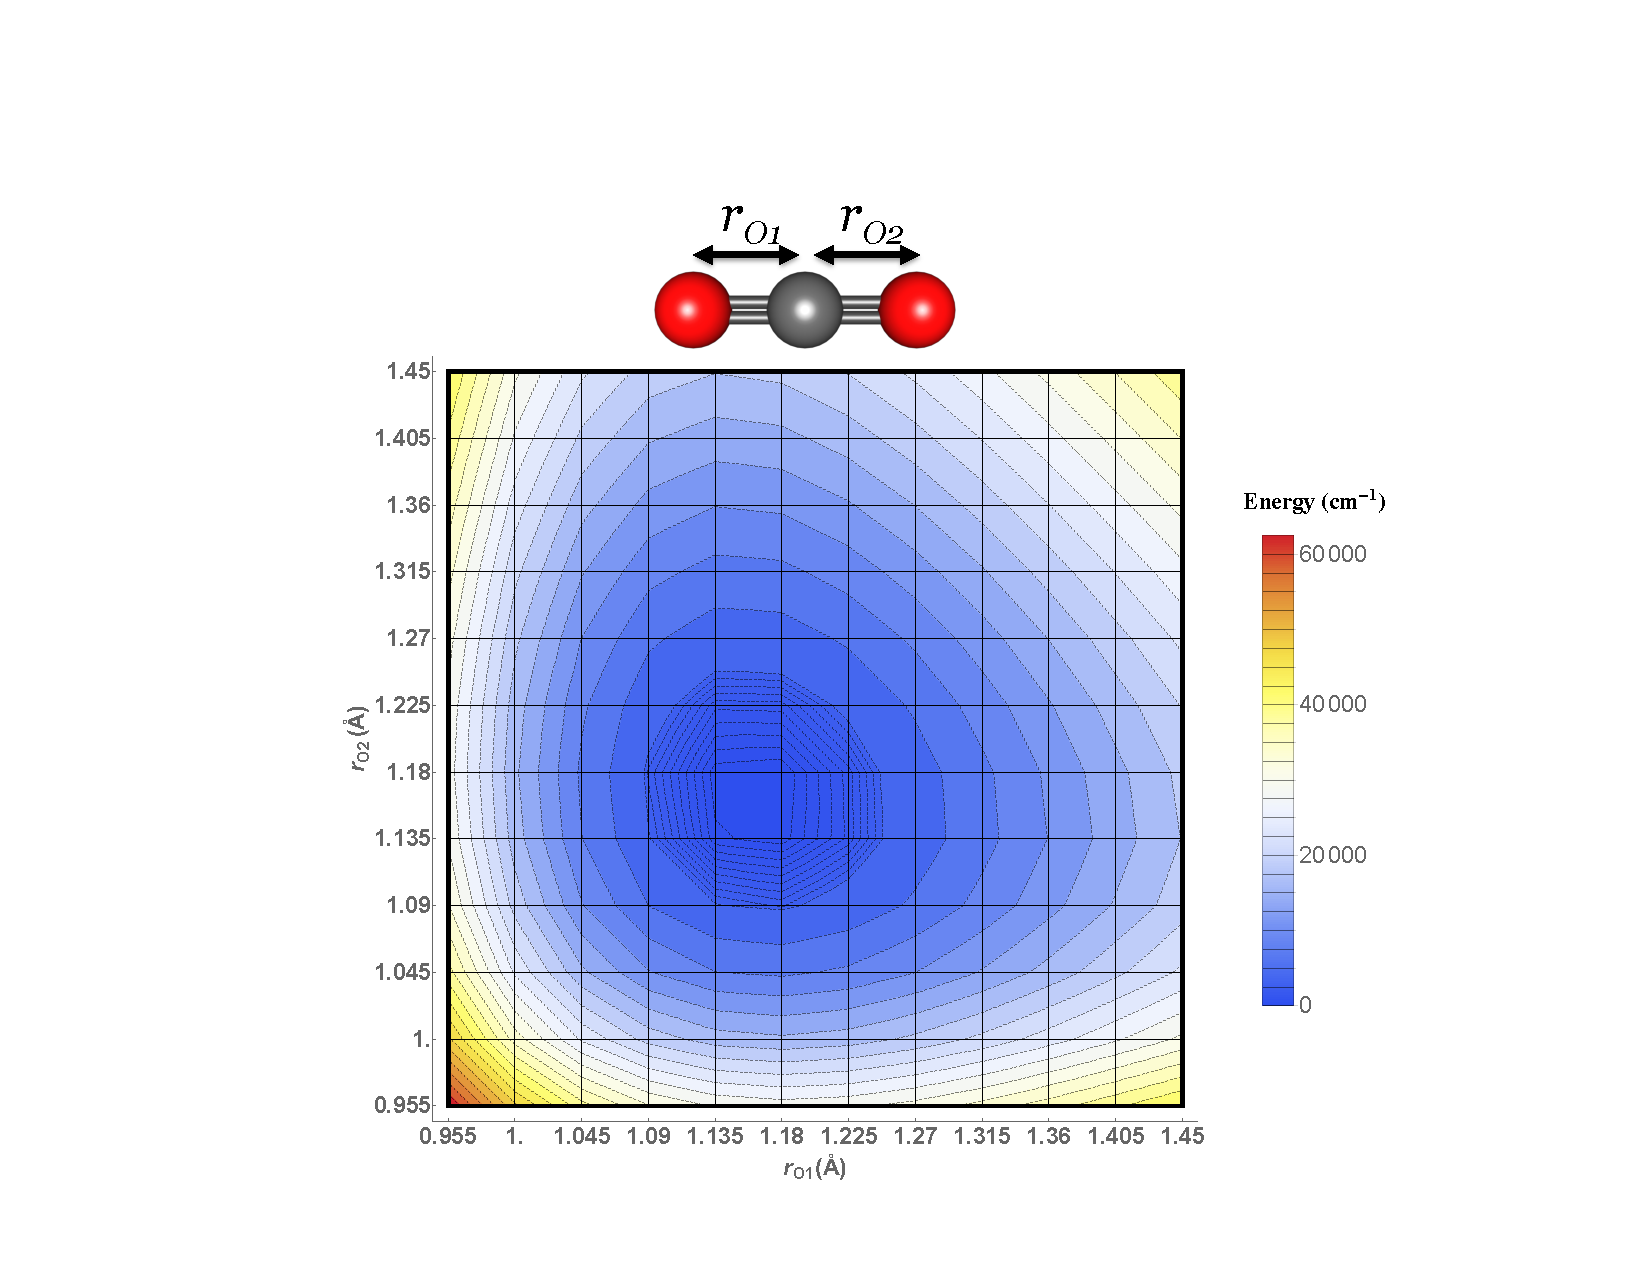
\includegraphics[width=\textwidth]{paper_02/Fig1.pdf}
  \caption[DVR contour plot]{Contour plot of a discrete variable representation (DVR) of the Born\textendash{}Oppenheimer potential energy surface of gas phase \ce{CO2}. Density functional theory single point energy calculations with the B3LYP functional and the 6-311++G(d,p) basis set were performed on carbon dioxide, incrementing each CO bond's length in steps of \SI{0.045}{\angstrom}, from \SIrange{0.955}{1.45}{\angstrom}. Below a relative energy of \SI{2500}{\wavenumber}, contour lines are spaced by \SI{100}{\wavenumber}, above they are spaced by \SI{2500}{\wavenumber}. Mesh intersections indicate individual single point energy calculations. In order to calculate vibrational frequencies, this potential energy surface is incorporated into a discretized version of the Hamiltonian for the stretching modes of \ce{CO2} (Eq.~\ref{paper_02:eq:1}), which is then numerically diagonalized. The asymmetric stretch frequency is obtained from the differences between the energy levels (Eq.~\ref{paper_02:eq:2}).}
  \label{paper_02:fig:1}
\end{figure}

\begin{figure}
  \centering
  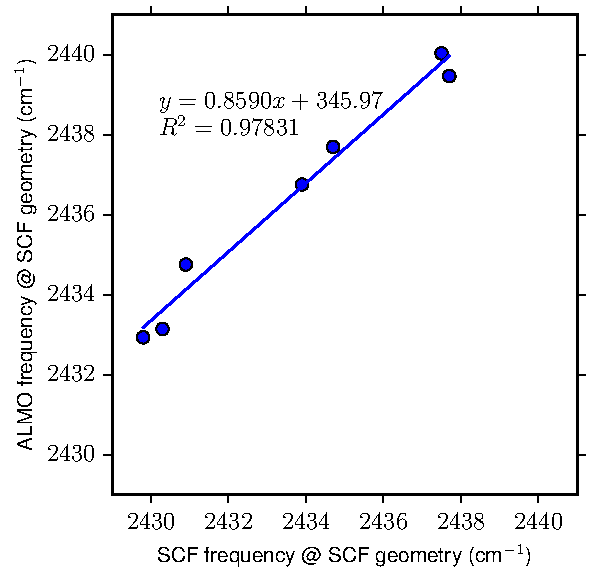
\includegraphics{paper_02/Fig2a.pdf}
  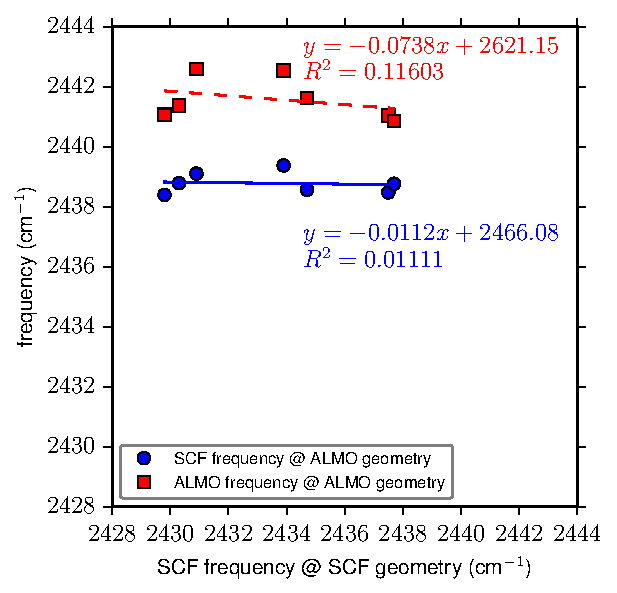
\includegraphics{paper_02/Fig2b.pdf}
  \caption{Comparison of B3LYP/SP frequencies calculated (a) within the ALMO (CT off) approach versus standard SCF (CT on) at the standard SCF-optimized geometry and (b) at the ALMO-optimized geometry versus standard SCF-optimized geometry with Hessian within the ALMO approach (red squares) versus Hessian using standard DFT (blue triangles). The frequencies are unscaled.}
  \label{paper_02:fig:2}
\end{figure}

\begin{figure}
  \centering
  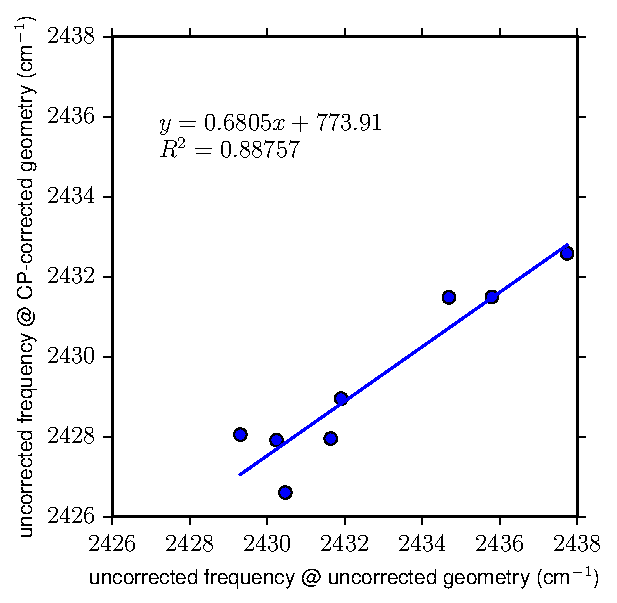
\includegraphics{paper_02/Fig3a.pdf}
  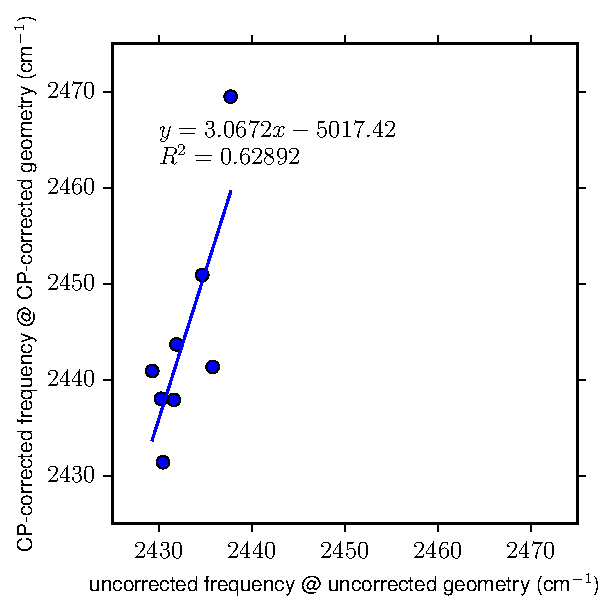
\includegraphics{paper_02/Fig3b.pdf}
  \caption{Comparison of B3LYP/SP frequencies (a) calculated at counterpoise (CP) corrected geometries versus uncorrected geometries and (b) calculated using CP-corrected Hessians at CP-corrected geometries versus uncorrected Hessians at uncorrected geometries. The frequencies are unscaled.}
  \label{paper_02:fig:3}
\end{figure}

\begin{figure}
  \centering
  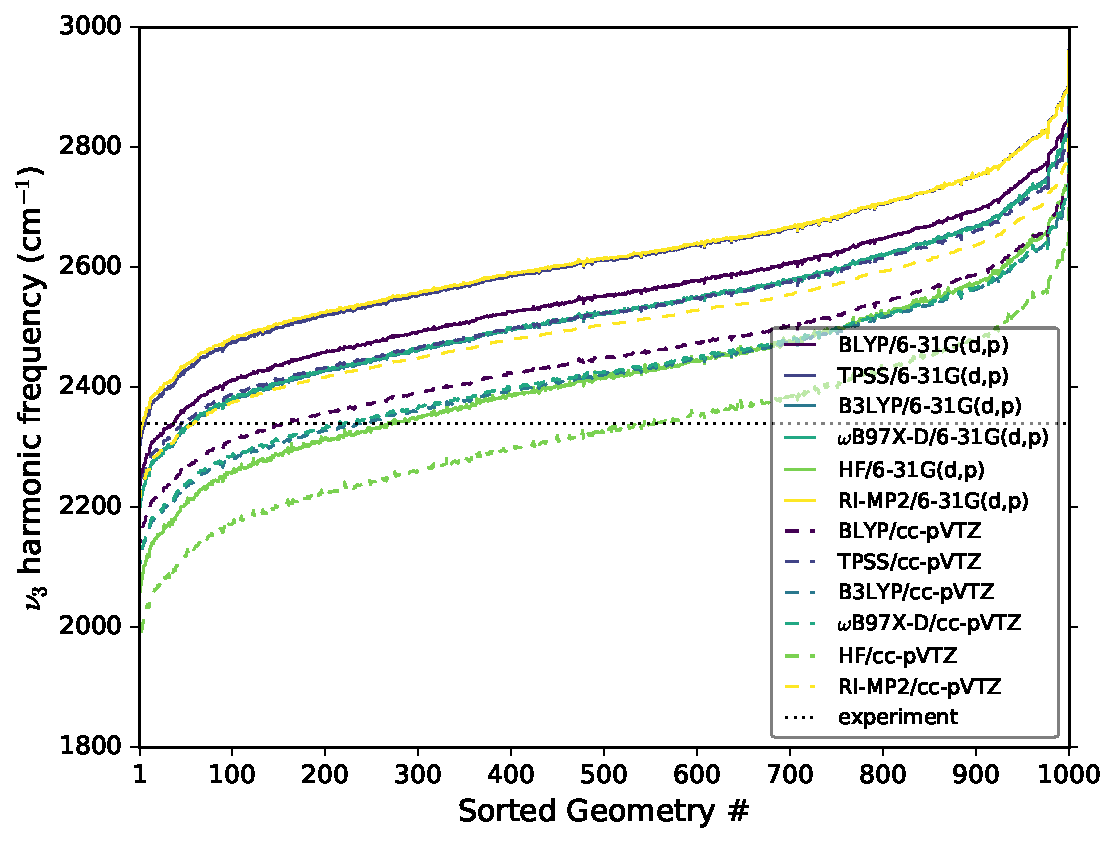
\includegraphics[width=\textwidth]{paper_02/Fig4.pdf}
  \caption{Dependence of harmonic \(\nu_3\) frequencies (unscaled) on the solvent box size (B3LYP/SP potential energy surface).}
  \label{paper_02:fig:4}
\end{figure}

\begin{figure}
  \centering
  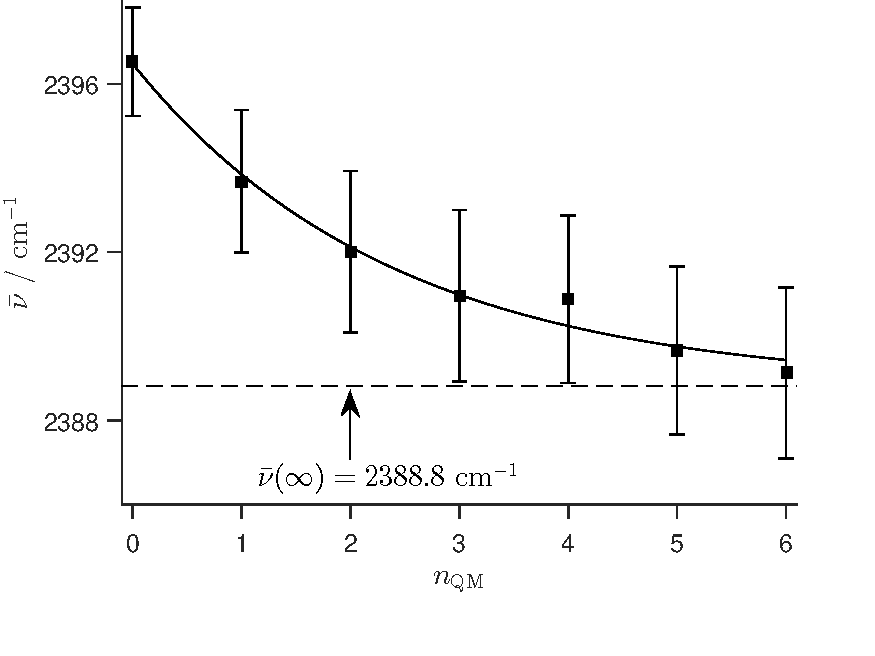
\includegraphics{paper_02/Fig5.pdf}
  \caption[DVR convergence with respect to number of QM ion pairs]{Dependence of DVR \(\nu_{3}\) mean frequency (\(\overline{\nu}\)) on the number of solvent ion pairs treated quantum mechanically (\(n_{QM}\)). Mean frequencies were calculated from \(N = 10\) representative MD snapshots using a B3LYP/SP potential energy surface. Error bars represent the standard deviation of the mean (\(SD_{\overline{x}} = \sigma_{x}/\sqrt{N}\)). The data were fitted to an exponential decay (\({\overline{\nu}}_{QM} = A\exp\left( - kn_{QM} \right) + {\overline{\nu}}_{converged}\)), with weights of \(1/SD_{\overline{x}}^{2}\) (\(R^2 = 0.99\)). The resulting estimate for the fully converged frequency at this level of theory is \(2388.8 \pm \SI{1.5}{\wavenumber}\).}
  \label{paper_02:fig:5}
\end{figure}

\begin{table}
  \centering
  \caption[Functional and basis set dependence of \ce{CO2} bond lengths]{Dependence of \(r_{\ce{O}1}\) and \(r_{\ce{O}1} + r_{\ce{O}2}\) bond lengths on functional (BLYP, B3LYP, and HF) and basis set (SP, LP, VDZ, VTZ, and VQZ) for a gas-phase cluster consisting of \ce{CO2} with a cation/anion pair.}
  \label{paper_02:tab:1}
  \begin{longtable}[]{@{}ccccccc@{}}
    \toprule
    & \(r_{\ce{O}1}\) (\si{\angstrom}) & \(r_{\ce{O}1} + r_{\ce{O}2}\) (\si{\angstrom}) \tabularnewline
    \midrule
    \endhead
    \ce{CO2} (free) & BLYP & B3LYP & HF & BLYP & B3LYP & HF\tabularnewline
    SP & 1.1828 & 1.1692 & 1.1433 & 2.3656 & 2.3383 & 2.2865\tabularnewline
    LP & 1.1744 & 1.1608 & 1.1357 & 2.3487 & 2.3216 & 2.2715\tabularnewline
    VDZ & 1.1815 & 1.1674 & 1.1406 & 2.3630 & 2.3348 & 2.2811\tabularnewline
    VTZ & 1.1736 & 1.1604 & 1.1362 & 2.3472 & 2.3208 & 2.2724\tabularnewline
    VQZ & 1.1720 & 1.1588 & 1.1345 & 2.3441 & 2.3176 & 2.2690\tabularnewline
    & \(r_{\ce{O}1}\) (\si{\angstrom}) & \(r_{\ce{O}1} + r_{\ce{O}2}\) (\si{\angstrom}) \tabularnewline
    \ce{CO2}/\ce{[BMIM][PF6]} & BLYP & B3LYP & HF & BLYP & B3LYP & HF\tabularnewline
    SP & 1.1854 & 1.1723 & 1.1473 & 2.3649 & 2.3380 & 2.2871\tabularnewline
    LP & 1.1775 & 1.1646 & 1.1402 & 2.3485 & 2.3217 & 2.2725\tabularnewline
    VDZ & 1.1845 & 1.1710 & 1.1450 & 2.3622 & 2.3345 & 2.2819\tabularnewline
    VTZ & 1.1766 & 1.1639 & 1.1402 & 2.3464 & 2.3204 & 2.2727\tabularnewline
    VQZ & 1.1749 & 1.1622 & 1.1385 & 2.3434 & 2.3173 & 2.2694\tabularnewline
    \bottomrule
  \end{longtable}
\end{table}

\begin{table}
  \centering
  \caption[Functional and basis set dependence of \ce{CO2} asymmetric stretch frequencies]{Dependence of \(\nu_3\) harmonic frequencies on functional (BLYP, B3LYP, and HF) and basis set (SP, LP, VDZ, VTZ, and VQZ) for an optimized gas-phase cluster consisting of \ce{CO2} and one cation/anion pair. All frequencies reported in \si{\wavenumber}. Reported frequencies are unscaled.}
  \label{paper_02:tab:2}
  \begin{longtable}[]{@{}cccc@{}}
    \toprule
    \begin{minipage}[b]{0.24\columnwidth}\raggedright
      Method

      Basis\strut
    \end{minipage} & \begin{minipage}[b]{0.24\columnwidth}\raggedright
      BLYP\strut
    \end{minipage} & \begin{minipage}[b]{0.24\columnwidth}\raggedright
      B3LYP\strut
    \end{minipage} & \begin{minipage}[b]{0.24\columnwidth}\raggedright
      HF\strut
    \end{minipage}\tabularnewline
    \midrule
    \endhead
    SP & 2348.88 & 2437.23 & 2582.87\tabularnewline
    LP & 2329.31 & 2419.80 & 2571.33\tabularnewline
    VDZ & 2332.11 & 2422.71 & 2577.29\tabularnewline
    VTZ & 2330.23 & 2417.28 & 2562.28\tabularnewline
    VQZ & 2322.26 & 2409.34 & 2553.85\tabularnewline
    \bottomrule
  \end{longtable}
\end{table}

\begin{table}
  \centering
  \caption[Charge transfer dependence of \ce{CO2} asymmetric stretch frequencies]{Dependence of CT contributions to the \(\nu_3\) frequency based on functional (BLYP, B3LYP, and HF) and basis set (SP, LP, VDZ, VTZ, and VQZ). Calculations are on an optimized gas-phase cluster of \ce{CO2} with a single cation/anion pair. All frequencies reported in \si{\wavenumber}. We distinguish two mechanisms by which CT can enter the frequency: (i) a ``geometry mechanism'' where CT determines the optimized geometry of the cluster, calculated as the difference between standard harmonic frequency results at the optimized standard (``CT on'') and ALMO (``CT off'') geometries. (ii) a ``curvature mechanism'' where CT enters by modifying the force constant at the optimized geometry, calculated as the difference between the ``CT on'' and ``CT off'' frequencies at the optimized standard (``CT on'') geometry.}
  \label{paper_02:tab:3}
  \begin{longtable}[]{@{}llll@{}}
    \toprule
    \begin{minipage}[b]{0.24\columnwidth}\raggedright
      \begin{enumerate}
        \def\labelenumi{(\roman{enumi})}
      \item
        \begin{quote}
          \textbf{``Geometry Mechanism'':}
        \end{quote}
      \end{enumerate}\strut
    \end{minipage}\tabularnewline
    \midrule
    \endhead
    \begin{minipage}[t]{0.24\columnwidth}\raggedright
      \textbf{Method}

      \textbf{Basis}\strut
    \end{minipage} & \begin{minipage}[t]{0.24\columnwidth}\raggedright
      BLYP\strut
    \end{minipage} & \begin{minipage}[t]{0.24\columnwidth}\raggedright
      B3LYP\strut
    \end{minipage} & \begin{minipage}[t]{0.24\columnwidth}\raggedright
      HF\strut
    \end{minipage}\tabularnewline
    6-31G(d,p) & -3.16 & -3.50 & -3.33\tabularnewline
    6-311++G(d,p) & -2.80 & -3.38 & -3.72\tabularnewline
    cc-pVDZ & -2.46 & -3.11 & -2.93\tabularnewline
    cc-pVTZ & -1.90 & -2.35 & -1.19\tabularnewline
    cc-pVQZ & -2.44 & N/A & N/A\tabularnewline
    \bottomrule
  \end{longtable}

  \begin{longtable}[]{@{}llll@{}}
    \toprule
    \begin{minipage}[b]{0.24\columnwidth}\raggedright
      \begin{enumerate}
        \def\labelenumi{(\roman{enumi})}
        \setcounter{enumi}{1}
      \item
        \begin{quote}
          \textbf{``Curvature Mechanism'':}
        \end{quote}
      \end{enumerate}\strut
    \end{minipage}\tabularnewline
    \midrule
    \endhead
    \begin{minipage}[t]{0.24\columnwidth}\raggedright
      \textbf{Method}

      \textbf{Basis}\strut
    \end{minipage} & \begin{minipage}[t]{0.24\columnwidth}\raggedright
      BLYP\strut
    \end{minipage} & \begin{minipage}[t]{0.24\columnwidth}\raggedright
      B3LYP\strut
    \end{minipage} & \begin{minipage}[t]{0.24\columnwidth}\raggedright
      HF\strut
    \end{minipage}\tabularnewline
    6-31G(d,p) & -2.72 & -2.86 & -2.80\tabularnewline
    6-311++G(d,p) & -1.31 & -1.25 & -1.55\tabularnewline
    cc-pVDZ & -2.92 & -2.97 & -2.53\tabularnewline
    cc-pVTZ & -1.43 & -1.33 & -0.94\tabularnewline
    cc-pVQZ & -1.18 & N/A & N/A\tabularnewline
    \bottomrule
  \end{longtable}
\end{table}

\begin{table}
  \centering
  \caption{Comparison of analytical harmonic (AH), grid-based harmonic (GH), and grid-based anharmonic (DVR) absolute \(\nu_3\) frequencies for \ce{CO2} in the gas phase (B3LYP/6-311++G(d,p) potential energy surface). Reported frequencies are unscaled.}
  \label{paper_02:tab:4}
  \begin{longtable}[]{@{}lcc@{}}
    \toprule
    & \(\nu_{3}\) (\si{\wavenumber}) & \(r_{\ce{OC}}\) (\si{\angstrom}) \tabularnewline
    \midrule
    \endhead
    analytical harmonic (AH) & 2420 & 1.161\tabularnewline
    grid-based harmonic (GH) & 2414 & 1.159\tabularnewline
    grid-based anharmonic (DVR) & 2384 & 1.165\tabularnewline
    \bottomrule
  \end{longtable}
\end{table}

\begin{table}
  \centering
  \caption{Summary of DVR data averaged from \num{85} MD snapshots (SP = small Pople = 6-31G(d,p), LP = large Pople = 6-311++G(d,p)) at the QM/MM level, treating \ce{CO2} plus \num{2} ion pairs quantum mechanically. Reported frequencies are unscaled.}
  \label{paper_02:tab:5}
  \begin{longtable}[]{@{}lllll@{}}
    \toprule
    PES & \(\nu_3\) (\si{\wavenumber}) & \(r_{\ce{O}1}\) (\si{\angstrom}) & \(r_{\ce{O}2}\) (\si{\angstrom}) & \(r_{\ce{O}1} + r_{\ce{O}2}\) (\si{\angstrom}) \tabularnewline
    \midrule
    \endhead
    B3LYP/SP, CT off & 2399.4 & 1.1724 & 1.1729 & 2.3454 \tabularnewline
    B3LYP/SP, CT on & 2389.5 & 1.1728 & 1.1734 & 2.3462 \tabularnewline
    B3LYP/LP, CT on & 2373.9 & 1.1645 & 1.1650 & 2.3295 \tabularnewline
    \bottomrule
  \end{longtable}
\end{table}

\begin{table}
  \centering
  \caption[Comparison of ALMO- versus SAPT0-decomposed interaction energies for MD clusters]{Comparison of ALMO- versus SAPT0-decomposed interaction energies averaged over \num{15} representative molecular dynamics snapshots. ALMO calculations were performed within the SP basis to allow comparison to results from Ref. 14. For SAPT0, we report both monomer-centered basis set (MCBS) and dimer-centered basis set (DCBS) results. Energies are reported in \si{\kcal\per\mole}.}
  \label{paper_02:tab:6}
  \begin{longtable}[]{@{}lllllll@{}}
    \toprule
    \begin{minipage}[b]{0.14\columnwidth}\raggedright
      \textbf{Component}\strut
    \end{minipage} & \begin{minipage}[b]{0.14\columnwidth}\raggedright
      \textbf{ALMO-DFT}

      6-31G**\strut
    \end{minipage} & \begin{minipage}[b]{0.14\columnwidth}\raggedright
      \textbf{ALMO-HF}

      6-31G**\strut
    \end{minipage} & \begin{minipage}[b]{0.14\columnwidth}\raggedright
      \textbf{SAPT0\\
      }SP\strut
    \end{minipage} & \begin{minipage}[b]{0.14\columnwidth}\raggedright
      \textbf{SAPT0\\
      }jun-cc-pVTZ\strut
    \end{minipage}\tabularnewline
    \midrule
    \endhead
    & & & MCBS & DCBS & MCBS & DCBS\tabularnewline
    \(E_{\text{el}}^{(10)}\) & \textemdash{} & \textemdash{} & -5.295 & -7.018 & -6.097 & -6.154\tabularnewline
    \(E_{\text{exch}}^{(10)}\) & \textemdash{} & \textemdash{} & 2.845 & 7.611 & 7.106 & 7.622\tabularnewline
    \(\mathbf{E_{\text{frz}}}\) & \textbf{0.500} & \textbf{0.082} & \textbf{-2.450} & \textbf{0.593} & \textbf{1.009} & \textbf{1.468}\tabularnewline
    \(E_{\text{ind}}^{(20)}\) & \textemdash{} & \textemdash{} & -1.218 & -3.636 & -2.593 & -3.916\tabularnewline
    \(E_{\text{ind-exch}}^{(20)}\) & \textemdash{} & \textemdash{} & 0.009 & 2.147 & 0.921 & 2.041\tabularnewline
    \(\delta_{\text{HF}}\) & \textemdash{} & \textemdash{} & -0.839 & -0.421 & -0.801 & -0.507\tabularnewline
    \(\mathbf{E_{\text{pol}}}\) & \textbf{-1.241} & \textbf{-1.303} & \textbf{-2.049} & \textbf{-1.910} & \textbf{-2.473} & \textbf{-2.382}\tabularnewline
    \(\mathbf{E_{\text{CT}}}\) & \textbf{-1.177} & \textbf{-0.102} & \textbf{-0.280} & \textbf{-0.203}\tabularnewline
    \(E_{\text{disp}}^{(20)}\) & \textemdash{} & \textemdash{} & -4.193 & -5.197 & -7.323 & -8.084\tabularnewline
    \(E_{\text{disp-exch}}^{(20)}\) & \textemdash{} & \textemdash{} & 0.058 & 0.483 & 0.393 & 0.671\tabularnewline
    \(\mathbf{E_{\text{disp}}}\) & \textbf{\textemdash{}} & \textbf{\textemdash{}} & \textbf{-4.135} & \textbf{-4.714} & \textbf{-6.930} & \textbf{-7.413}\tabularnewline
    \(\mathbf{E_{\text{int}}}\) & \textbf{-1.918} & \textbf{-1.323} & \textbf{-8.634} & \textbf{-6.031} & \textbf{-8.394} & \textbf{-8.326}\tabularnewline
    \bottomrule
  \end{longtable}
\end{table}

\begin{table}
  \centering
  \caption{Correlation coefficients (\(R^2\)) between different solute-solvent interaction energy components as calculated at the ALMO-DFT (B3LYP), ALMO-HF, and SAPT0 level within the SP basis. (a) Comparison between individual components and the total interaction energy (\(E_{\text{tot}}\)) calculated for each methodology. (b) Correlation coefficients between contributions to the \ce{CO2}\textendash{}IL interaction energy calculated via ALMO as compared to the corresponding SAPT0 energy terms. Reported SAPT0 results are within the dimer-centered basis set (DCBS), except for the charge transfer component, which is calculated as the difference between monomer- and dimer-centered basis set results for the induction energy.}
  \label{paper_02:tab:7}

  (a)

  \begin{longtable}[]{@{}cccc@{}}
    \toprule
    Component & ALMO-DFT & ALMO-HF & SAPT0\tabularnewline
    \midrule
    \endhead
    \(E_{\text{frz}}\) & 0.887 & 0.944 & 0.870 (\(E_{\text{el}}\): 0.602, \(E_{\text{exch}}\): 0.073) \tabularnewline
    \(E_{\text{pol}}\) & 0.170 & 0.087 & 0.073\tabularnewline
    \(E_{\text{CT}}\) & 0.225 & 0.270 & 0.093\tabularnewline
    \(E_{\text{disp}}\) & \textemdash{} & \textemdash{} & 0.150\tabularnewline
    \bottomrule
  \end{longtable}

  (b)

  \begin{longtable}[]{@{}lcc@{}}
    \toprule
    Component (ALMO \textemdash{} SAPT0) & ALMO-DFT & ALMO-HF\tabularnewline
    \midrule
    \endhead
    \(E_{\text{frz}}\) \textemdash{} \(E_{\text{el}} + E_{\text{exch}}\) & 0.989 & 0.993\tabularnewline
    \(E_{\text{pol}}\) \textemdash{} \(E_{\text{ind}} + E_{\text{ind-exch}} + \delta_{\text{HF}}\) & 0.887 & 0.927\tabularnewline
    \(E_{\text{CT}}\) \textemdash{} \(E_{\text{CT}}\) & 0.720 & 0.383\tabularnewline
    \(E_{\text{tot}}\) \textemdash{} \(E_{\text{tot}}\) & 0.913 & 0.927\tabularnewline
    \bottomrule
  \end{longtable}
\end{table}

ASSOCIATED CONTENT

\textbf{Supporting Information}. Statistics on calculated harmonic frequencies across different MD snapshots, bin sizes and weights for 15-25 representative structures sampled from MD snapshots, as well as XYZ coordinates of MD snapshots.

AUTHOR INFORMATION

Corresponding Author

* Author to whom correspondence should be addressed: \href{mailto:lambrecht@pitt.edu}{\nolinkurl{lambrecht@pitt.edu}}

Author Contributions

The manuscript was written through contributions of all authors. All authors have given approval to the final version of the manuscript.

Funding Sources

SAC is grateful for financial support from the National Science Foundation (CHE-1565471), the American Chemical Society Petroleum Research Fund (52648-ND6), and the Sustainable Energy Initiative at the University of Notre Dame. This material is based upon work supported by the National Science Foundation under Grant No. (CHE-1454105). TAB acknowledges support of the Pittsburgh Quantum Institute. DSL thanks the University of Pittsburgh for start-up funding.

ACKNOWLEDGMENT

EJB thanks Dr. Mary Sherman for performing initial SAPT calculations and cclib\cite{OBoyle2008,Berquist2015} for the analysis framework. The authors thank Prof. Kenneth D. Jordan for helpful discussions. SAC and CAD are also thankful for high-performance computing resources and support from the Center for Research Computing at the University of Notre Dame.~EJB and DSL thank the Center for Simulation and Modeling at the University of Pittsburgh for providing computational resources.

\subsection{Table of Contents Graphic}
\label{table-of-contents-graphic}

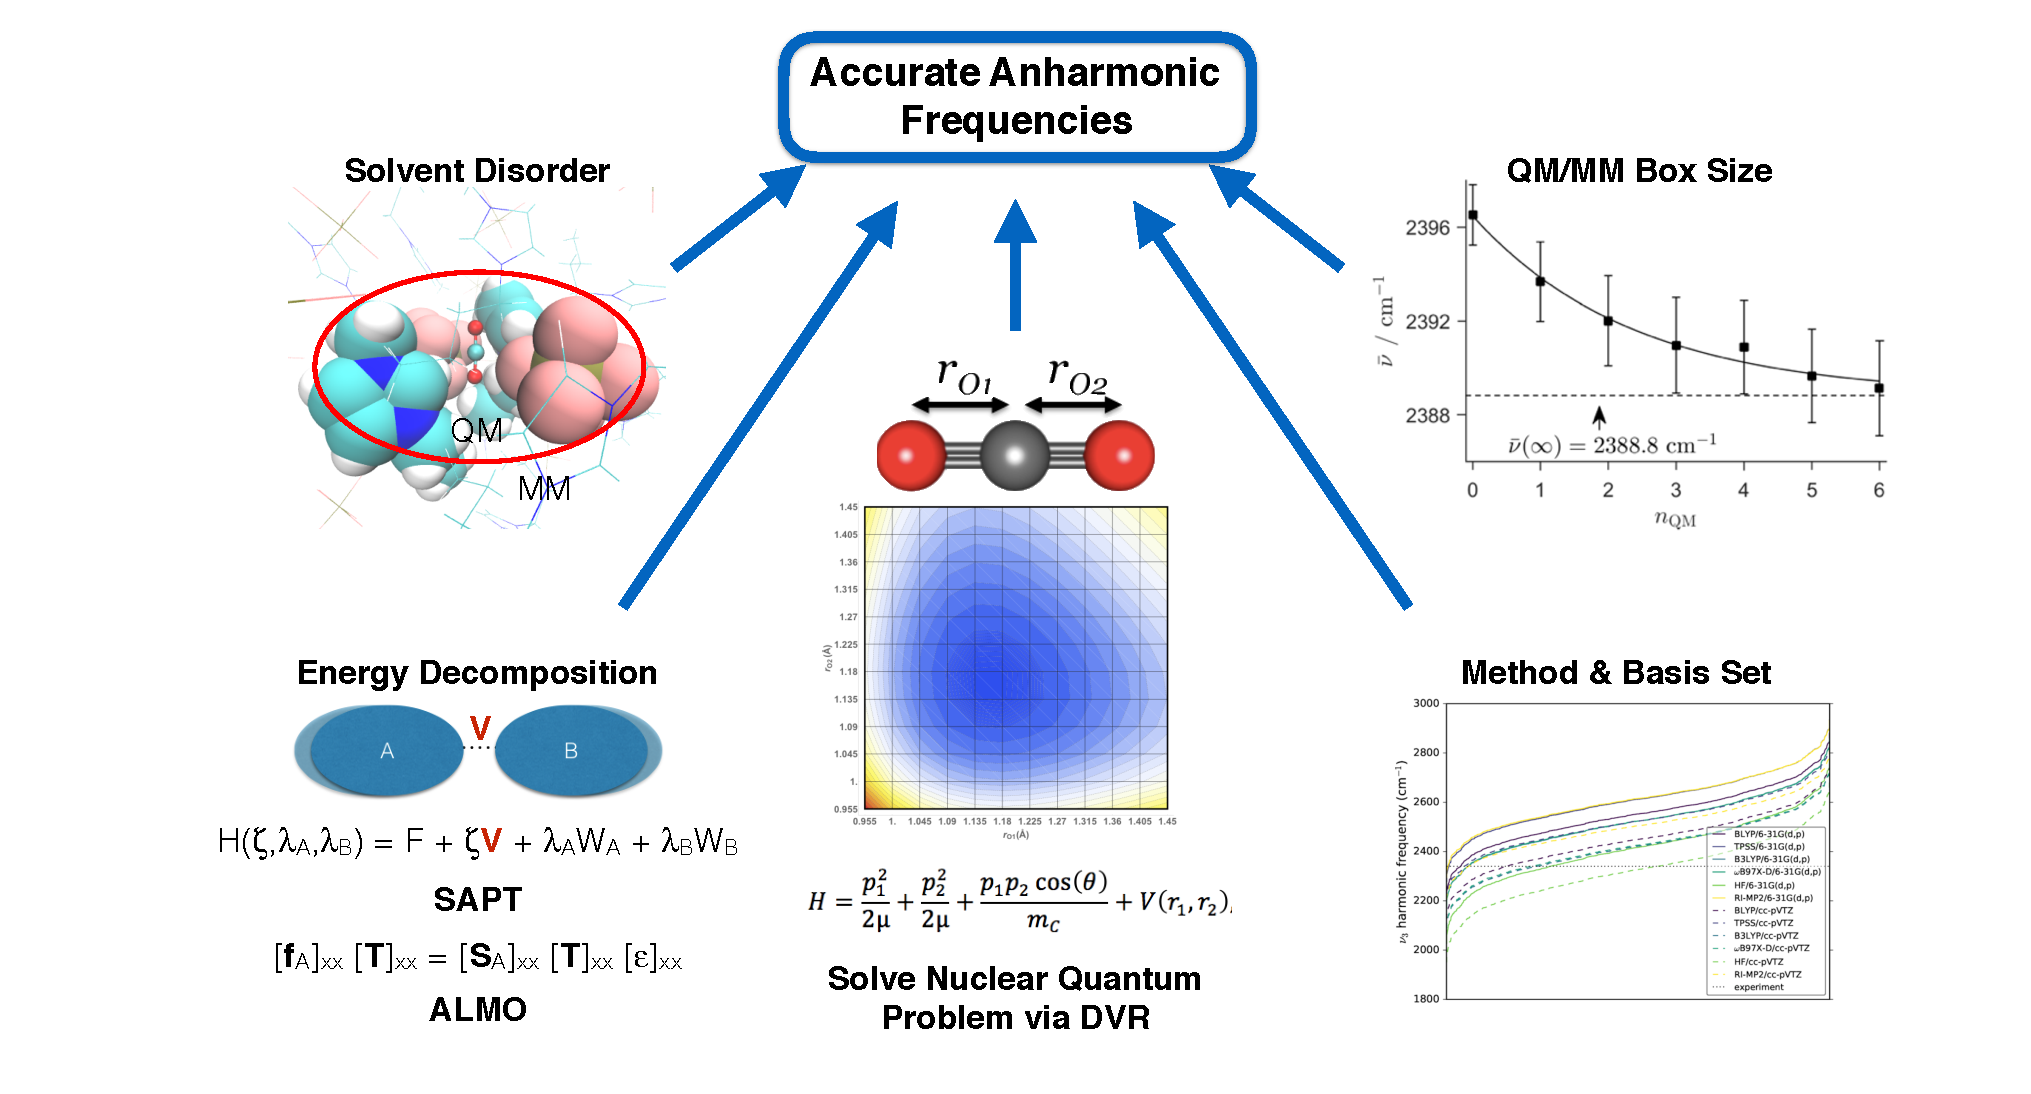
\includegraphics[width=\textwidth]{paper_02/TOC.pdf}

\section{\caps{Statistical Distribution of Harmonic Frequencies for MD snapshots}}
\label{paper_02:sec:SI}

\begin{table}[h]
  \centering
  \caption[Descriptive statistics for \ce{CO2} asymmetric stretch frequencies from MD]{Statistics for dependence of \ce{CO2} asymmetric stretch frequencies on quantum chemical method and basis set dependence on \num{1000} MD snapshots, 0 QM/256 MM. All frequencies in \si{\wavenumber}.}
  \label{paper_02:tab:S1}
  \begin{longtable}[]{@{}lllllllll@{}}
    \toprule
    \textbf{method} & \textbf{basis set} & \textbf{min} & \textbf{max} & \textbf{range} & \textbf{mean} & \textbf{median} & \textbf{standard deviation (population)} & \textbf{standard deviation (sample)}\tabularnewline
    \midrule
    \endhead
    BLYP & 6-31G(d,p) & 2179.26 & 2915.23 & 735.97 & 2551.84 & 2552.16 & 112.92 & 112.86\tabularnewline
    TPSS & 6-31G(d,p) & 2247.16 & 2967.72 & 720.56 & 2611.68 & 2612.06 & 110.39 & 110.33\tabularnewline
    B3LYP & 6-31G(d,p) & 2141.31 & 2892.22 & 750.91 & 2522.55 & 2522.96 & 115.09 & 115.03\tabularnewline
    \(\omega\)B97X-D & 6-31G(d,p) & 2138.86 & 2894.15 & 755.29 & 2523.38 & 2523.93 & 114.14 & 114.08\tabularnewline
    HF & 6-31G(d,p) & 1990.89 & 2814.31 & 823.42 & 2415.50 & 2416.41 & 125.46 & 125.40\tabularnewline
    RI-MP2 & 6-31G(d,p) & 2264.73 & 2964.82 & 700.09 & 2615.07 & 2615.27 & 107.68 & 107.62\tabularnewline
    BLYP & cc-pVTZ & 2083.99 & 2802.55 & 718.56 & 2448.66 & 2449.17 & 110.15 & 110.10\tabularnewline
    TPSS & cc-pVTZ & 2164.75 & 2871.70 & 706.95 & 2523.22 & 2523.74 & 108.27 & 108.22\tabularnewline
    B3LYP & cc-pVTZ & 2047.30 & 2781.22 & 733.92 & 2420.89 & 2421.51 & 112.37 & 112.31\tabularnewline
    \(\omega\)B97X-D & cc-pVTZ & 2048.35 & 2787.24 & 738.89 & 2425.06 & 2425.52 & 111.67 & 111.61\tabularnewline
    HF & cc-pVTZ & 1908.93 & 2714.98 & 806.05 & 2325.54 & 2326.49 & 122.60 & 122.54\tabularnewline
    RI-MP2 & cc-pVTZ & 2165.68 & 2842.63 & 676.95 & 2504.51 & 2504.63 & 104.39 & 104.34\tabularnewline
    \bottomrule
  \end{longtable}
\end{table}

\section{\caps{Histogram and Weights of Frequency Distributions from MD Snapshots}}
\label{paper_02:sec:SII}

\begin{table}[h]
  \centering
  \caption{Weights and bin counts for each quantum chemical method and basis set, 0 QM/256 MM. Weights from B3LYP/6-31(d,p) are used for selecting the structures for box size dependence and SAPT calculations.}
  \label{paper_02:tab:S2}
  \begin{longtable}[]{@{}llllll@{}}
    \toprule
    \begin{minipage}[b]{0.16\columnwidth}\raggedright
      \textbf{method}\strut
    \end{minipage} & \begin{minipage}[b]{0.16\columnwidth}\raggedright
      \textbf{basis set}\strut
    \end{minipage} & \begin{minipage}[b]{0.16\columnwidth}\raggedright
      \textbf{bin edges}\strut
    \end{minipage} & \begin{minipage}[b]{0.16\columnwidth}\raggedright
      \textbf{histogram}\strut
    \end{minipage} & \begin{minipage}[b]{0.16\columnwidth}\raggedright
      \textbf{weights}\strut
    \end{minipage} & \begin{minipage}[b]{0.16\columnwidth}\raggedright
      \textbf{Sum (histogram)}\strut
    \end{minipage}\tabularnewline
    \midrule
    \endhead
    BLYP & 6-31G(d,p) & {[}2269.54 2382.46 2495.38 2608.30 2721.23 2834.13{]} & {[} 59 245 398 224 64{]} & {[} 0.05959596 0.24747475 0.40202020 0.22626263 0.06464646{]} & 990\tabularnewline
    TPSS & 6-31G(d,p) & {[}2335.71 2446.10 2556.49 2666.88 2777.27 2887.66{]} & {[} 59 244 400 223 64{]} & {[} 0.05959596 0.24646465 0.40404040 0.22525253 0.06464646{]} & 990\tabularnewline
    B3LYP & 6-31G(d,p) & {[}2234.82 2349.91 2465.00 2580.09 2695.18 2810.27{]} & {[} 59 245 398 224 64{]} & {[} 0.05959596 0.24747475 0.40202020 0.22626263 0.06464646{]} & 990\tabularnewline
    \(\omega\)B97X-D & 6-31G(d,p) & {[}2238.04 2352.18 2466.31 2580.45 2694.59 2808.72{]} & {[} 57 241 401 225 63{]} & {[} 0.05775076 0.24417427 0.40628166 0.22796353 0.06382979{]} & 987\tabularnewline
    HF & 6-31G(d,p) & {[}2101.85 2227.31 2352.77 2478.23 2603.69 2729.15{]} & {[} 61 240 399 228 63{]} & {[} 0.06155399 0.24217962 0.40262361 0.23007064 0.06357215{]} & 991\tabularnewline
    RI-MP2 & 6-31G(d,p) & {[}2345.88 2453.56 2561.23 2668.91 2776.58 2884.26{]} & {[} 59 246 398 223 64{]} & {[} 0.05959596 0.24848485 0.40202020 0.22525253 0.06464646{]} & 990\tabularnewline
    BLYP & cc-pVTZ & {[}2173.29 2283.44 2393.59 2503.74 2613.89 2724.04{]} & {[} 59 245 398 224 64{]} & {[} 0.05959596 0.24747475 0.40202020 0.22626263 0.06464646{]} & 990\tabularnewline
    TPSS & cc-pVTZ & {[}2252.54 2360.81 2469.09 2577.36 2685.64 2793.91{]} & {[} 59 245 396 226 64{]} & {[} 0.05959596 0.24747475 0.40000000 0.22828283 0.06464646{]} & 990\tabularnewline
    B3LYP & cc-pVTZ & {[}2139.97 2252.34 2364.70 2477.07 2589.44 2701.80{]} & {[} 59 244 399 224 64{]} & {[} 0.05959596 0.24646465 0.40303030 0.22626263 0.06464646{]} & 990\tabularnewline
    \(\omega\)B97X-D & cc-pVTZ & {[}2145.89 2257.56 2369.22 2480.89 2592.56 2704.22{]} & {[} 57 243 399 225 63{]} & {[} 0.05775076 0.24620061 0.40425532 0.22796353 0.06382979{]} & 987\tabularnewline
    HF & cc-pVTZ & {[}2019.04 2141.64 2264.24 2386.84 2509.44 2632.04{]} & {[} 61 240 401 226 63{]} & {[} 0.06155399 0.24217962 0.40464178 0.22805247 0.06357215{]} & 991\tabularnewline
    RI-MP2 & cc-pVTZ & {[}2243.53 2347.92 2452.32 2556.71 2661.11 2765.50{]} & {[} 59 247 394 226 64{]} & {[} 0.05959596 0.24949495 0.39797980 0.22828283 0.06464646{]} & 990\tabularnewline
    \bottomrule
  \end{longtable}
\end{table}

\section{\caps{Method and Basis Set Dependence of Harmonic Frequencies}}
\label{paper_02:sec:SIII}

It is imperative to investigate how sensitive the prediction of relative trends is with respect to the computational approach. To this end, we consider snapshots from MD simulations (see Ref. {[}paper II{]} for details), which allow us to test how well different computational approaches can predict \emph{trends} in dependence of the local coordination environment around the \ce{CO2} and the bulk solvent structure. Fig.~\ref{paper_02:fig:S3} shows the \ce{CO2} \(\nu_{3}\) harmonic frequencies calculated for \num{1000} statistically uncorrelated MD snapshots (0 QM/256 MM) using various SCF-type approaches, as compared to Møller-Plesset perturbation theory to second order (MP2) as the least expensive wave function-based method that incorporates dispersion effects.\cite{WCMS:WCMS58} The predicted harmonic frequencies in Fig.~\ref{paper_02:fig:S3} are parallel to each other for most of the frequency range, independent of method and basis set choice. In fact, there is almost complete overlap between the B3LYP/SP and \(\omega\)B97X-D/SP distributions, and to a lesser degree for B3LYP/VTZ and \(\omega\)B97X-D/VTZ. There is minor crossing of curves in two instances, 1. TPSS/VTZ with \(\omega\)B97X-D/SP, and 2. HF/SP with both B3LYP/VTZ and \(\omega\)B97X-D/VTZ, but nevertheless the conservation of qualitative trends seems excellent. The ordering of calculated frequencies is, from smallest to largest, HF, B3LYP, \(\omega\)B97X-D, BLYP, TPSS, and MP2, using the SP basis set. Within the VTZ basis, the ordering of MP2 and TPSS is interchanged. As expected, the MP2 results are most sensitive to the basis set size, as wave-function based correlation methods require larger basis sets for convergence compared to self-consistent field approaches (HF and DFT). The VTZ basis set predicts frequency distributions that are red-shifted compared to the SP basis set, in agreement with the trends observed from Table~\ref{paper_02:tab:2}.

These results for relative trends in vibrational frequencies are highly encouraging. Aside from a multiplicative scaling factor, any of the common quantum chemical methods investigated here can qualitatively reproduce the distribution of harmonic frequencies. The similarity in performance between B3LYP and \(\omega\)B97X-D is somewhat surprising, as the former is a global hybrid with a fixed fraction of HF exchange over all interelectronic distances, and \(\omega\)B97X-D is a range-separated functional with a variable fraction of HF exchange. An explanation of this observation will be provided together with the SAPT results.

\begin{figure}[h]
  \centering
  % \includegraphics[width=6in,height=4.52222in]{media/image1.emf}
  \caption{Harmonic \(\nu_{3}\) frequencies (unscaled) for different methods and basis sets, ordered from lowest to highest frequency according to MP2/VTZ (0 QM/256 MM). The TPSS meta-GGA\cite{Tao2003} and the \(\omega\)B97X-D\cite{Chai2008} hybrid GGA density functionals are included as representatives of more recent functionals. \(\omega\)B97X-D is both a range-separated functional, with a minimum 22\% HF exchange at \(r_{e} = 0\), increasing smoothly to 100\% as \(r_{e} \rightarrow \infty\), and it includes an empirical dispersion correction. To aid in recognizing trends, we have ordered the structures by increasing MP2/VTZ frequency. MP2 calculations use the resolution of the identity (RI) approximation\cite{Feyereisen1993,Weigend1997,Distasio2007} and the cc-pVQZ-RI fitting basis set\cite{Weigend2002}.}
  \label{paper_02:fig:S3}
\end{figure}

To confirm that the good agreement in relative trends is not an artifact of the reordering, \ce{CO2} \(\nu_{3}\) harmonic frequencies for the first \num{50} of \num{1000} MD snapshots are shown in Fig.~\ref{paper_02:fig:S4} (0 QM/256 MM, VTZ basis set). Although there are large absolute jumps between snapshots due to the \SI{50}{\pico\second} time step between them, the ordering between quantum chemical methods does not change, and the gaps between each method are constant.

\begin{figure}[h]
  \centering
  % \includegraphics[width=6in,height=4.59097in]{media/image2.emf}
  \caption{Harmonic \(\nu_{3}\) frequencies (unscaled) for the first \num{50} (out of \num{1000}) snapshots calculated with different methods and the cc-pVTZ basis set (0 QM/256 MM).}
  \label{paper_02:fig:S4}
\end{figure}

\begin{table}[h]
  \centering
  \caption[Effect of empirical and self-consistent dispersion corrections in ALMO-EDA]{Effect of empirical and self-consistent dispersion corrections on ALMO-decomposed interaction energies with comparison to SAPT0. Values are weighted averages over the same \num{15} snapshots as in Table~\ref{paper_02:tab:6}. Energies are reported in \si{\kcal\per\mole}.}
  \label{paper_02:tab:S3}
  \begin{longtable}[]{@{}lccccc@{}}
    \toprule
    \textbf{Method} & \(\mathbf{E_{frz}}\) & \(\mathbf{E_{pol}}\) & \(\mathbf{E_{CT}}\) & \(\mathbf{E_{disp}}\) & \(\mathbf{E_{tot}}\)\tabularnewline
    \midrule
    \endhead
    HF/6-31G(d,p) & 0.082 & -1.303 & -0.102 & \textemdash{} & -1.323\tabularnewline
    B3LYP/6-31G(d,p) & 0.500 & -1.241 & -1.177 & \textemdash{} & -1.918\tabularnewline
    B3LYP-D2/6-31G(d,p) & 0.500 & -1.241 & -1.177 & -6.269 & -8.187\tabularnewline
    B3LYP-D3/6-31G(d,p) & 0.500 & -1.241 & -1.177 & -6.464 & -8.382\tabularnewline
    \(\omega\)B97X-D/6-31G(d,p) & -3.343 & -1.245 & -1.168 & \textemdash{} & -5.757\tabularnewline
    \(\omega\)B97X-D/cc-pVTZ & -3.114 & -1.617 & -1.209 & \textemdash{} & -5.941\tabularnewline
    \(\omega\)B97M-V/6-31G(d,p) & -5.494 & -1.256 & -0.523 & \textemdash{} & -7.274\tabularnewline
    \(\omega\)B97M-V/cc-pVTZ & -5.149 & -1.649 & -0.889 & \textemdash{} & -7.687\tabularnewline
    SAPT0/6-31G(d,p)/MCBS & -2.450 & -2.049 & -0.280 & -4.135 & -8.634\tabularnewline
    SAPT0/6-31G(d,p)/DCBS & 0.593 & -1.910 & & -4.714 & -6.031\tabularnewline
    SAPT0/jun-cc-pVTZ/MCBS & 1.009 & -2.473 & -0.203 & -6.930 & -8.394\tabularnewline
    SAPT0/jun-cc-pVTZ/DCBS & 1.469 & -2.382 & & -7.413 & -8.326\tabularnewline
    \bottomrule
  \end{longtable}
\end{table}

\section{\caps{Solvatochromic Shift Dependence on Counterpoise Corrections}}
\label{paper_02:sec:SIV}

\begin{table}
  \centering
  \caption[Effect of counterpoise correction on \ce{CO2} asymmetric stretch frequency]{Effect of counterpoise correction on \ce{CO2} \(\nu_3\) harmonic frequency when applied during geometry optimization and/or the harmonic frequency calculation. Clusters are with 1 \ce{CO2}, 1 MMIM cation, and 1 anion. All frequencies are in \si{\wavenumber} and unscaled. The first column is from our previous paper. CP-corrected calculations were performed using Cuby as a driver for Turbomole 6.6 at the B3LYP/SP level with numerical integration grid 7.}
  \label{paper_02:tab:S4}
  CP-correction for geometry? / CP-correction for frequencies?
  \begin{longtable}[]{@{}lllll@{}}
    \toprule
    \textbf{Anion} & \textbf{no/no} & \textbf{yes/no} & \textbf{no/yes} & \textbf{yes/yes}\tabularnewline
    \midrule
    \endhead
    \ce{TFA} & 2429.31 & 2428.05 & 2457.238 & 2440.879\tabularnewline
    \ce{SCN} (\ce{S}-coordinated) & 2430.24 & 2427.91 & 2445.642 & 2438.003\tabularnewline
    \ce{DCA} & 2430.47 & 2426.60 & 2436.113 & 2431.383\tabularnewline
    \ce{SCN} (\ce{N}-coordinated) & 2431.64 & 2427.95 & 2432.691 & 2437.876\tabularnewline
    \ce{TfO} & 2431.91 & 2428.95 & 2441.921 & 2443.665\tabularnewline
    \ce{BF4} & 2434.69 & 2431.48 & 2454.767 & 2450.890\tabularnewline
    \ce{Tf2N} & 2435.80 & 2431.49 & 2451.851 & 2441.309\tabularnewline
    \ce{PF6} & 2437.74 & 2432.58 & 2479.806 & 2469.473\tabularnewline
    \bottomrule
  \end{longtable}
\end{table}

\section{\caps{Potential Energy Surface Fitting}}
\label{paper_02:sec:SV}

We fitted the discrete variable representation (DVR) of the Born-Oppenheimer potential energy surface of gas phase \ce{CO2} to a vibrational potential expanded in the local modes basis using a nonlinear least squares method. The potential energy expansion was truncated at fourth order, and off-diagonal fourth order terms (e.g.  \(c_{3}[(x - x_{0})^{2}(y - y_{0})^{2}]\)) were omitted, using the following form:

% \begin{dmath*}
\begin{equation*}
  V( x,y ) = a_{1}( x - x_{0} )^{2} + a_{2}( y - y_{0} )^{2} + a_{3}( x - x_{0} )( y - y_{0} ) + b_{1}( x - x_{0} )^{3} + b_{2}( y - y_{0} )^{3} + b_{3}[ ( x - x_{0} )^{2}( y - y_{0} ) + ( x - x_{0} )( y - y_{0} )^{2} ] + c_{1}( x - x_{0} )^{4} + c_{2}( y - y_{0} )^{4}
\end{equation*}

The resulting fit to the data was excellent (\(R^2 = 0.9997\)).

The force constants and internal coordinates were calculated (the F matrix) and multiplied by the appropriate mass weighting (G matrix). The product was diagonalized to obtain eigenvalues and eigenvectors, which give the normal modes and frequencies of the symmetric stretch (\(\nu_{1} = \SI{1377}{\wavenumber}\)) and antisymmetric stretch (\(\nu_{3} = \SI{2414}{\wavenumber}\)).

\begin{table}
  \centering
  \caption{Best fit parameters for DVR representation of the gas phase \ce{CO2} potential energy surface.}
  \label{paper_02:tab:S5}
  \begin{longtable}[]{@{}ll@{}}
    \toprule
    Coefficient Name & Value (with 95\% confidence bound)\tabularnewline
    \midrule
    \endhead
    \(a_1\) & \(1.8834 \pm 0.0178\) \si{\hartree\per\angstrom\squared}\tabularnewline
    \(a_2\) & \(1.8834 \pm 0.0178\) \si{\hartree\per\angstrom\squared}\tabularnewline
    \(a_3\) & \(0.3305 \pm 0.0087\) \si{\hartree\per\angstrom\squared}\tabularnewline
    \(b_1\) & \(-5.0013 \pm 0.1124\) \si{\hartree\per\angstrom\cubed}\tabularnewline
    \(b_2\) & \(-5.0005 \pm 0.1123\) \si{\hartree\per\angstrom\cubed}\tabularnewline
    \(b_3\) & \(-0.2205 \pm 0.0330\) \si{\hartree\per\angstrom\cubed}\tabularnewline
    \(c_1\) & \(6.3508 \pm 0.4031\) \si{\hartree\per\angstrom\tothe{4}}\tabularnewline
    \(c_2\) & \(6.3485 \pm 0.4031\) \si{\hartree\per\angstrom\tothe{4}}\tabularnewline
    \(x_0\) & \(1.1594 \pm 0.0009\) \si{\angstrom}\tabularnewline
    \(y_0\) & \(1.1594 \pm 0.0009\) \si{\angstrom}\tabularnewline
    \bottomrule
  \end{longtable}
\end{table}

\section{\caps{\(\nu_{3}\) Frequency Convergence with Increasing QM Size}}
\label{paper_02:sec:SVI}

To test the qualitative accuracy of the calculations using smaller QM regions, we examined the correlation between frequencies calculated with \(n = 0-5\) QM pairs and \num{6} QM pairs for each snapshot. The data were fitted using a linear regression analysis.

\begin{table}
  \centering
  \caption{Fitting results for correlation of QM/MM harmonic frequencies of \num{10} MD snapshots, with increasing numbers of anion-cation pairs (\(n_{\text{QM}}\)) treated quantum mechanically.}
  \label{paper_02:tab:S6}
  \begin{longtable}[]{@{}ccc@{}}
    \toprule
    \(n_{\text{QM}}(1)\) & \(n_{\text{QM}}(2)\) & Fitting Results\tabularnewline
    \midrule
    \endhead
    \begin{minipage}[t]{0.32\columnwidth}\raggedright
      0\strut
    \end{minipage} & \begin{minipage}[t]{0.32\columnwidth}\raggedright
      6\strut
    \end{minipage} & \begin{minipage}[t]{0.32\columnwidth}\raggedright
      \textbf{Estimate Standard Error}
      \textbf{Intercept} -20.915 1024.4
      \textbf{Slope} 1.0056 0.42745
      \textbf{Root Mean Squared Error:} 5.52
      \textbf{R-squared:} 0.409, \textbf{Adjusted R-Squared} 0.335\strut
    \end{minipage}\tabularnewline
    \begin{minipage}[t]{0.32\columnwidth}\raggedright
      1\strut
    \end{minipage} & \begin{minipage}[t]{0.32\columnwidth}\raggedright
      6\strut
    \end{minipage} & \begin{minipage}[t]{0.32\columnwidth}\raggedright
      \textbf{Estimate Standard Error}
      \textbf{Intercept} 60.512 593.34
      \textbf{Slope} 0.97282 0.24788
      \textbf{Root Mean Squared Error:} 4.2
      \textbf{R-squared:} 0.658, \textbf{Adjusted R-Squared} 0.615\strut
    \end{minipage}\tabularnewline
    \begin{minipage}[t]{0.32\columnwidth}\raggedright
      2\strut
    \end{minipage} & \begin{minipage}[t]{0.32\columnwidth}\raggedright
      6\strut
    \end{minipage} & \begin{minipage}[t]{0.32\columnwidth}\raggedright
      \textbf{Estimate Standard Error}
      \textbf{Intercept} 98.181 384
      \textbf{Slope} 0.95775 0.16053
      \textbf{Root Mean Squared Error:} 3.08
      \textbf{R-squared:} 0.816, \textbf{Adjusted R-Squared} 0.794\strut
    \end{minipage}\tabularnewline
    \begin{minipage}[t]{0.32\columnwidth}\raggedright
      3\strut
    \end{minipage} & \begin{minipage}[t]{0.32\columnwidth}\raggedright
      6\strut
    \end{minipage} & \begin{minipage}[t]{0.32\columnwidth}\raggedright
      \textbf{Estimate Standard Error}
      \textbf{Intercept} 173.5 306.89
      \textbf{Slope} 0.92667 0.12835
      \textbf{Root Mean Squared Error:} 2.62
      \textbf{R-squared:} 0.867, \textbf{Adjusted R-Squared} 0.85\strut
    \end{minipage}\tabularnewline
    \begin{minipage}[t]{0.32\columnwidth}\raggedright
      4\strut
    \end{minipage} & \begin{minipage}[t]{0.32\columnwidth}\raggedright
      6\strut
    \end{minipage} & \begin{minipage}[t]{0.32\columnwidth}\raggedright
      \textbf{Estimate Standard Error}
      \textbf{Intercept} 2.1463 172.16
      \textbf{Slope} 0.99837 0.072008
      \textbf{Root Mean Squared Error:} 1.44
      \textbf{R-squared:} 0.96, \textbf{Adjusted R-Squared} 0.955\strut
    \end{minipage}\tabularnewline
    \begin{minipage}[t]{0.32\columnwidth}\raggedright
      5\strut
    \end{minipage} & \begin{minipage}[t]{0.32\columnwidth}\raggedright
      6\strut
    \end{minipage} & \begin{minipage}[t]{0.32\columnwidth}\raggedright
      \textbf{Estimate Standard Error}
      \textbf{Intercept} -26.98 85.681
      \textbf{Slope} 1.0111 0.035855
      \textbf{Root Mean Squared Error:} 0.717
      \textbf{R-squared:} 0.99, \textbf{Adjusted R-Squared} 0.989\strut
    \end{minipage}\tabularnewline
    \bottomrule
  \end{longtable}
\end{table}

\begin{figure}
  \centering
  % \includegraphics[width=5.27in,height=8in]{media/image3.png}
  \caption{Correlation plots for QM/MM harmonic frequencies of \num{10} MD snapshots, with increasing numbers of anion-cation pairs treated quantum mechanically.}
  \label{paper_02:fig:S5}
\end{figure}
